%% ===========================================================================
%% Propose, then judge -- manuscript (Elsevier CAS template)
%% Template: Elsevier CAS bundle v2.4, single column (cas-sc), see gabarit/cas-sc-template.tex
%% Build (from docs/article/): pdflatex main && bibtex main && pdflatex main && pdflatex main
%% All results are final test-set results (frozen protocol, docs/protocole_test.md); missing items in \todo{...}.
%% ===========================================================================
\documentclass[a4paper,fleqn]{cas-sc}
% If the front matter runs over more than one page:
%\documentclass[a4paper,fleqn,longmktitle]{cas-sc}

\usepackage[authoryear,longnamesfirst]{natbib}

%% Vector fonts for the sans-serif and typewriter families. The class sets the text in STIX but
%% leaves these two families on Computer Modern (cmss, and cmtt when Inconsolata is missing),
%% which T1 encoding turns into bitmap EC fonts. Latin Modern (package lm, vector Type 1)
%% replaces them; the main text stays in STIX, as in the template. (A plain \usepackage{lmodern}
%% would also replace STIX for the text.)
\renewcommand{\sfdefault}{lmss}
\renewcommand{\ttdefault}{lmtt}
\setlength{\emergencystretch}{2em}   % lets lines with long \texttt names break instead of overflowing

%% Already loaded by cas-sc.cls / cas-common.sty (do NOT load again):
%%   graphicx, amsmath, amsfonts, amssymb, booktabs, makecell, multirow, array,
%%   colortbl, dcolumn, xspace, xcolor[svgnames,dvipsnames], hyperref[colorlinks],
%%   fontenc[T1], stix fonts, etoolbox, xparse.
%% enumitem is deliberately NOT used: cas-common redefines itemize/enumerate.
\usepackage{siunitx}
\usepackage{pgfplots}
\pgfplotsset{compat=1.18}
\usepackage[capitalise,noabbrev]{cleveref}   % after hyperref (loaded by the class)

\sisetup{group-separator={,},group-minimum-digits=4}

%% ---------------------------------------------------------------------------
%% Draft macros
%% \prov{x}: provisional number (development set); shown in colour so that every
%%           value still to be replaced by the frozen test-set run is visible.
%% \todo{x}: missing result, reference or author decision.
%% Set \provfinaltrue before the final build to print \prov values in black.
%% ---------------------------------------------------------------------------
\definecolor{provcolor}{RGB}{0,90,181}
\definecolor{todocolor}{RGB}{200,0,0}
\newif\ifprovfinal
\provfinalfalse
\newcommand{\prov}[1]{\ifprovfinal#1\else\textcolor{provcolor}{#1}\fi}
\newcommand{\todo}[1]{\textcolor{todocolor}{\textbf{[TODO:} #1\textbf{]}}}
\newcommand{\provnote}{Provisional, development set.\xspace}

%% Notation
\newcommand{\none}{\ensuremath{\bot}}
\newcommand{\Cand}{\ensuremath{\mathcal{C}}}

%% Figures generated by experiments/figures.py (pgfplots .tex + .dat).
%% All figures live in figures/ (relative to this folder): diagrams (PDF) and result plots (pgfplots).
\newcommand{\figdir}{figures}   % diagrams (PDF) and result figures (pgfplots .tex/.dat), all inside the article folder
\pgfplotsset{table/search path={\figdir}}
\newcommand{\genfigure}[2]{%
  \IfFileExists{\figdir/#1.tex}{\input{\figdir/#1.tex}}{%
    \fbox{\parbox{0.85\linewidth}{\centering\footnotesize
      \todo{figure \texttt{#1.tex} not generated yet: run
      \texttt{python -m experiments.figures --split test --out docs/article/figures}; #2}}}}}

%% Total of pages in the footer ("Page x of N"): cas-common.sty writes \thepage at \end{document} BEFORE the
%% pending floats are flushed, so N was too small (28 for 30 pages). We flush them first and write the real last
%% page; this later \csxdef overrides the class's one when the .aux is read. Compile twice.
\makeatletter
\AtEndDocument{\clearpage\immediate\write\@auxout{\string\csxdef{lastpage}{\the\numexpr\value{page}-1\relax}}}
\makeatother

\begin{document}
\let\WriteBookmarks\relax
\def\floatpagepagefraction{1}
\def\textpagefraction{.001}

\shorttitle{Propose, then judge: small calibrated judges versus LLM judges}
\shortauthors{C. Cruz, H. Ghanem and H. Cherifi}

%% Proposed title (no abbreviations, as required by the guide for authors).
\title[mode = title]{Propose, then judge: a small calibrated decision model versus large language model judges for multilingual slot filling}
%% Alternative 1: When to act and when to ask: small fine-tuned judges are more accurate, cheaper and better calibrated than large language model judges
%% Alternative 2: Knowing when to ask: calibrated candidate selection with a compact decision model in hybrid dialogue systems

\author[1]{Christophe Cruz}[orcid=0000-0002-5611-9479]  % ORCID from the public registry: to be confirmed by the author
\cormark[1]
\ead{christophe.cruz@ube.fr}
%% CRediT roles (authors, 1 Nov 2026): the idea is C. Cruz's; development and writing were shared.
\credit{Conceptualization, Methodology, Software, Validation, Formal analysis, Investigation, Data curation, Writing -- original draft, Writing -- review \& editing, Visualization, Project administration, Funding acquisition}

\author[1]{Hussam Ghanem}[orcid=0009-0002-2652-5748]  % ORCID from the public registry (Université Bourgogne Europe)
\ead{hussam.ghanem@ube.fr}
\credit{Methodology, Software, Validation, Formal analysis, Investigation, Data curation, Writing -- original draft, Writing -- review \& editing, Visualization}

\author[1]{Hocine Cherifi}[orcid=0000-0001-9124-4921]  % ORCID from the public registry (ICB UMR 6303)
\ead{hocine.cherifi@ube.fr}
\credit{Methodology, Software, Validation, Formal analysis, Investigation, Data curation, Writing -- original draft, Writing -- review \& editing, Visualization}

%% Affiliation and postal address from the ICB website: to be confirmed by the author (NOTES.md).
\affiliation[1]{organization={Laboratoire Interdisciplinaire Carnot de Bourgogne (ICB), UMR 6303 CNRS, Université Bourgogne Europe},
            addressline={9 avenue Alain Savary, BP 47870},
            city={Dijon Cedex},
            postcode={21078},
            country={France}}

\cortext[1]{Corresponding author}

\begin{abstract}
% Word count (macros stripped, checked by script): see NOTES.md. Limit: 350.
Large language models are increasingly used as judges that pick one answer among options, but they are costly and their confidence rarely tells when a system may act on its own. We study this question in a hybrid architecture for task-oriented dialogue: inexpensive extractors propose candidate values for each slot, and a judge either selects one candidate or abstains. We compare Laya, a compact non-autoregressive decision model with fewer than half a billion parameters, used zero-shot and fine-tuned with a strictly proper scoring rule, against three open-weight large language model judges of 27 to 180 billion parameters on the same options, and against a fine-tuned sequence tagger. We cover three public benchmarks (MultiATIS++, MTOP and Multi3WOZ), English and French, single- and multi-turn inputs, and oracle and real candidate lists, with several seeds and Holm-corrected paired tests. With oracle candidates, the fine-tuned judge reaches a test slot F1 of 0.92--0.95, against 0.38--0.84 for the best large model, and all 72 paired comparisons of F1 and false positives favour it. Most of the gap comes from abstention: large models fill 15--21\% of the slots that the user did not express on MultiATIS++, against 0.4--0.5\% for the fine-tuned judge. Per request, it is 3 to 6 times faster, on a fraction of one GPU. After temperature scaling, its confidences rank its errors far better, with an area under the risk--coverage curve 3 to 40 times lower; at a 5\% risk it decides 39--100\% of the requests without asking, whereas no large model exceeds 1\% on MTOP. The judge is, however, only as good as its candidates: when slot values are literal spans of the utterance, the tagger alone outperforms the whole pipeline with our proposers (F1 0.83--0.95 against 0.63--0.83), whereas the pipeline wins on multi-turn dialogue, where values come from the history or must be mapped to canonical forms. Augmenting the option lists during training makes the judge robust to longer lists and missing values only when it mimics realistic confusions between slots. A small calibrated judge is thus a practical decision component for hybrid systems, provided that its proposers are strong.
\end{abstract}

%% Graphical abstract (encouraged): candidate = figures/architecture.pdf (or a simplified version of it).
%\begin{graphicalabstract}
%\includegraphics{}
%\end{graphicalabstract}

%% Same text as highlights.txt (3-5 bullets, <= 85 characters each; checked by script).
\begin{highlights}
\item A small fine-tuned judge beats 27B-180B LLM judges at choosing slot values
\item LLM judges fail mainly by answering when the user expressed no value
\item The small judge's confidences rank its errors far better: lower AURC
\item A plain BIO tagger beats the pipeline when slot values are literal spans
\item List augmentation helps only when it mimics real confusions between slots
\end{highlights}

\begin{keywords}
Small language models \sep
Large language model judges \sep
Calibration \sep
Selective prediction \sep
Slot filling \sep
Multilingual dialogue systems \sep
Abstention
\end{keywords}

\maketitle

%% ===========================================================================
\section{Introduction}
\label{sec:intro}
%% ===========================================================================

Large language models (LLMs) are now routinely asked to act as \emph{judges}: given a context and a short list of options, they return the option they find best. This pattern underlies LLM-as-a-judge evaluation \citep{zheng2023mtbench,liu2023geval}, tool and function selection \citep{li2024fnctod}, and many agentic pipelines in which a model must decide whether to act, to do nothing, or to ask for clarification. Two properties matter as much as accuracy in such settings. The first is \emph{cost}: a judge sits inside an interactive loop and is called many times per user turn. The second is \emph{trustworthy confidence}: a system can act autonomously only if the judge's probability tells it reliably when it is likely to be wrong, so that uncertain cases can be deferred to the user or to a more expensive component \citep{geifman2017selective}. LLM judges are known to be sensitive to the order and labels of options \citep{wang2024fair,li2025calibraeval}, and their confidence must often be recalibrated before it can be used \citep{radharapu2026calibrating}.

This paper asks whether a small decision model, fine-tuned for the judging role and calibrated, can replace an open-weight LLM judge in such a loop. We study the question on a concrete and well-instrumented task: \emph{slot filling} in task-oriented dialogue. For a request such as ``a flight from \emph{Lyon} to \emph{Paris} on \emph{Thursday morning}'', the system must fill each slot of the current intent (departure city, arrival city, date, time\ldots) with the value expressed by the user, or leave it empty. Recent work relies on generative LLMs for this task \citep{hu2022icdst,heck2023chatgpt,li2024fnctod}. Generation is flexible, but it is costly, it can produce values that do not occur in the input, and the resulting scores are rarely usable to decide whether to act.

We instead separate two roles, following a long line of picklist-based dialogue state trackers \citep{lee2019sumbt,zhang2020dsdst} and of retrieve-then-rerank pipelines \citep{wu2020blink}:
\begin{enumerate}
  \item \textbf{Propose.} Inexpensive generators (a lexicon of training values, a zero-shot span extractor such as GLiNER \citep{zaratiana2024gliner}, the ontology, the dialogue history) build, for each slot, a short list of candidate values from the current context.
  \item \textbf{Judge.} A light judge either selects one candidate or answers ``not specified''. Its probability, once calibrated, drives a three-zone decision: \emph{act} (fill the slot), \emph{ignore} (leave it empty), or \emph{ask} (defer).
\end{enumerate}
Because the judge can only return one of the proposed candidates or abstain, it cannot hallucinate a value. Its errors therefore decompose cleanly into \emph{candidate recall} (the right value was never proposed), \emph{choice} (it was proposed but not selected) and \emph{abstention} (a value was selected for a slot the user did not express), which makes the architecture convenient to diagnose.

As the judge we use Laya \citep{laya2026}, a publicly released, non-autoregressive ``System~1'' decision model built on modern bidirectional encoders \citep{warner2025modernbert,marone2026mmbert}, which answers multiple-choice questions about a structured state in a single forward pass. We compare it, zero-shot and after fine-tuning, with three recent open-weight LLM judges of 27 to 180 billion parameters from two families \citep{qwen38,qwen38flashnext,gemma4report}, all prompted with the same options and scored from the log-probabilities of their first answer token. The evaluation spans three public benchmarks with complementary properties: MultiATIS++ \citep{xu2020multiatis} (one domain, single turn), MTOP \citep{li2021mtop} (eleven domains and many intents, single turn) and Multi3WOZ \citep{hu2023multi3woz} (multi-domain, multi-turn dialogue), in English and in French, with both oracle candidate lists (to measure the judge alone) and real ones (to measure the whole pipeline).

The general-AI question behind this setting is the trade-off between a large general model used zero-shot and a small model specialised for one decision. Recent studies show that small fine-tuned models can match or beat LLMs on classification and slot filling once a modest amount of labelled data is available \citep{pecher2025comparing,aguirre2025finetuning,rana2025zeroshot}. We add two dimensions that matter for deployment and that these studies do not measure: whether the judge \emph{knows when it does not know} (risk--coverage behaviour after calibration), and how robust it is when the shape of its input changes (list length, missing gold value, language).

\paragraph{Research questions} We organise the study around five questions:
\textbf{RQ1} (efficiency) Does a fine-tuned Laya judge approach an open-weight LLM judge in slot F1, at a much lower cost?
\textbf{RQ2} (decomposition) Which share of the error comes from candidate recall, and which from the choice, and how do they vary with the number of candidates $k$ and the rate of missing gold values?
\textbf{RQ3} (generalisation) Does the judge transfer from English to French?
\textbf{RQ4} (abstention) Do calibration and the decision rule yield a useful risk--coverage trade-off?
\textbf{RQ5} (training) Does random augmentation of the option lists at training time make the judge robust to a changing context?

\paragraph{Contributions}
\begin{enumerate}
  \item A \textbf{proposer--judge formulation} of slot filling as calibrated candidate selection with explicit abstention, and a reproducible conversion of three span-annotated benchmarks (two languages, single- and multi-turn) into this format, including a domain filter for multi-turn dialogue (\cref{sec:method,sec:setup}).
  \item A \textbf{fine-tuning recipe} for a non-autoregressive decision model: supervised optimisation of the log score on training items produced by the inference code itself, so that training and evaluation cannot differ in format, with checkpoint selection on development F1 and an \emph{option-list augmentation} designed to reproduce the confusions of real candidate generators (\cref{sec:method}).
  \item A \textbf{controlled comparison with three open-weight LLM judges} (27--180\,B parameters, two families) on identical inputs: the fine-tuned judge is more accurate on every benchmark, language and candidate type, 3 to 6 times faster per request and 5 to 38 times faster in batch throughput, mainly because it abstains correctly (\cref{sec:rq1}).
  \item A \textbf{reliability analysis} showing that after calibration the small judge's confidences rank its errors far better than those of the LLMs (area under the risk--coverage curve 3 to 40 times lower), so that it can decide most requests without asking at a few percent risk, which none of the LLM judges can do on MTOP (\cref{sec:rq4}).
  \item A \textbf{comparison with a fine-tuned sequence tagger} that delimits where the proposer--judge architecture pays off: the tagger alone is better when slot values are literal spans of the utterance, the pipeline when values come from the dialogue history or must be mapped to canonical forms; the judge itself is not the bottleneck, the proposers are (\cref{sec:rq2-tagger}).
  \item An \textbf{error decomposition and robustness study} across candidate recall, choice and abstention, list size, missing values and cross-lingual transfer, with a negative-then-corrected result on augmentation that shows \emph{which} augmentation helps (\cref{sec:rq2,sec:rq3,sec:rq5}), all under a reproducibility protocol with multiple seeds, cluster bootstrap intervals, Holm-corrected paired permutation tests and code fingerprints in every run (\cref{sec:stats}).
\end{enumerate}

The rest of the paper is organised as follows. \Cref{sec:related} reviews related work. \Cref{sec:method} formalises the proposer--judge architecture and describes the judges, the candidate generators, fine-tuning, augmentation and the calibrated decision. \Cref{sec:setup} details datasets, conditions, metrics and the statistical protocol. \Cref{sec:results} answers RQ1--RQ5, \cref{sec:discussion} discusses errors, cost, calibration, limitations and threats to validity, and \cref{sec:conclusion} concludes.


%% ===========================================================================
\section{Related work}
\label{sec:related}
%% ===========================================================================

Our work sits at the crossing of five lines of research: natural language understanding (NLU) and dialogue state tracking, schema-guided and LLM-based approaches, LLMs as judges, candidate generation followed by selection, and calibration and selective prediction. A last paragraph positions it within the recent comparisons of small and large models.

\paragraph{Joint intent and slot models, and multilingual NLU}
Slot filling is classically cast as sequence labelling on top of a pre-trained encoder, jointly with intent classification \citep{chen2019jointbert}. Multilingual benchmarks extend this setting to many languages: MultiATIS++ \citep{xu2020multiatis}, distributed by the Linguistic Data Consortium as \emph{ATIS -- Seven Languages} \citep{mansour2021atis7}, MTOP \citep{li2021mtop} and MASSIVE \citep{fitzgerald2023massive}. These works provide our datasets and the cross-lingual protocols (train in English and test in another language, train in the target language, train on both). Sequence labellers are the natural proposers of our architecture and our extraction baseline (C0, \cref{sec:rq2-tagger}).

\paragraph{Dialogue state tracking: choosing versus extracting}
Multi-domain dialogue state tracking has long opposed two strategies. Picklist approaches score every value of a fixed ontology, as in SUMBT \citep{lee2019sumbt}; span or generation approaches extract or generate the value, as in TRADE \citep{wu2019trade}; DS-DST combines both, picking categorical slots from a list and extracting non-categorical ones \citep{zhang2020dsdst}. Our judge is a direct descendant of picklist tracking, with two differences: candidates are built \emph{per request} from the current context instead of a fixed ontology, and the judge is a generic decision model that receives the slot description as text rather than a slot-specific classifier. Multilingual multi-turn data remain scarce; Multi3WOZ \citep{hu2023multi3woz} and X-RiSAWOZ \citep{moradshahi2023xrisawoz} provide culturally adapted dialogues, and we use the former for French multi-turn evaluation.

\paragraph{Schema-guided and LLM-based slot filling}
Describing slots in natural language enables zero-shot transfer to unseen services: the Schema-Guided Dialogue dataset \citep{rastogi2020sgd}, slot descriptions for generative trackers \citep{lin2021t5dst} and description-driven modelling \citep{zhao2022d3st}; SGD-X measures robustness to paraphrased schemas \citep{lee2022sgdx}. With LLMs, dialogue state tracking became an in-context learning \citep{hu2022icdst}, zero-shot prompting \citep{heck2023chatgpt} or function-calling \citep{li2024fnctod} problem. Routing between small and large models reduces cost \citep{lee2024orchestrallm}, and bounded neuro-symbolic agents validate state updates with a symbolic checker to avoid hallucinated values \citep{lin2026reactod}. We share the motivation of predictability with the latter, but we enforce it by construction: the judge never generates a value. Our slot descriptions also follow the schema-guided tradition; robustness to renamed or paraphrased schemas in the spirit of SGD-X is left for future work (\cref{sec:limitations}).

\paragraph{LLMs as judges and their biases}
LLM-as-a-judge evaluation correlates well with human preferences \citep{zheng2023mtbench,liu2023geval}, but LLM judges suffer from position bias and are not fair evaluators by default \citep{wang2024fair}; permuting option positions or identifiers changes their decisions, which can be partly corrected by recalibrating the prediction distribution \citep{li2025calibraeval}. Linear probes on hidden states give better calibrated judges than verbalised confidence \citep{radharapu2026calibrating}. Our setting differs from evaluation: the judge acts \emph{online}, inside the system, and its probability is used to decide whether to act. We use neutral letter keys, shuffle the options with a fixed seed for every judge, and read probabilities from first-token log-probabilities, which makes the LLM judge directly comparable to the decision model.

\paragraph{Generate, then select}
Entity linking pipelines retrieve candidates and then rerank them with a cross-encoder \citep{wu2020blink}; zero-shot text classification can be cast as entailment between the input and a verbalised label \citep{yin2019benchmarking}; GLiNER extracts entity spans for arbitrary label descriptions with a bidirectional encoder \citep{zaratiana2024gliner}. Our architecture applies the same ``generate cheaply, select carefully'' principle to slot values, with GLiNER as one of the proposers.

\paragraph{Calibration and selective prediction}
Modern networks are often over-confident; temperature scaling \citep{guo2017calibration} and isotonic regression \citep{zadrozny2002transforming} are simple post-hoc corrections. Selective classification lets a model abstain below a confidence threshold and characterises the trade-off by a risk--coverage curve \citep{geifman2017selective}. Strictly proper scoring rules such as the log score reward honest probabilities \citep{gneiting2007scoring}; Laya's original training uses rewards based on such rules \citep{laya2026}, and we fine-tune it with the log score directly. Our three-zone decision (act, ignore, ask) is a selective-prediction policy whose threshold is set on development data for a target risk.

\paragraph{Small specialised models versus large general models}
Several recent studies compare fine-tuned small models with general LLMs. Around one hundred labelled examples suffice on average for a specialised small model to match a general LLM in text classification, although variance raises this number substantially \citep{pecher2025comparing}. In slot filling, a fine-tuned medium-size LLM outperforms zero-shot GPT-4o and JointBERT on MASSIVE \citep{aguirre2025finetuning}, black-box distillation into a small model beats LLMs on industrial call-centre data \citep{rana2025zeroshot}, and small-model predictions can be injected into an LLM prompt to improve cross-domain zero-shot slot filling \citep{li2025synergistic}. Closest to our decision rule, \citet{tikhomirov2026selection} show that when an encoder forwards only its uncertain cases, a compact LLM verifier does not improve the cost--quality frontier, and that confidence gating on the encoder is preferable. Compared with these works, our judge is an order of magnitude smaller than the smallest LLMs considered (under half a billion parameters), the comparison is made on identical candidate lists with the same option format, and we evaluate the reliability of confidences (risk--coverage) and robustness to the shape of the input, in two languages and in multi-turn dialogue.

\todo{Literature search beyond the ACL Anthology titles (arXiv, Semantic Scholar, SIGDIAL, TALN), as noted in docs/etat\_de\_l\_art.md; add any work combining French, multi-turn and cost--accuracy--abstention analysis.}

%% ===========================================================================
\section{Problem formulation and method}
\label{sec:method}
%% ===========================================================================

\subsection{Proposer--judge formulation}
\label{sec:formulation}

\begin{figure}[pos=t]
\centering
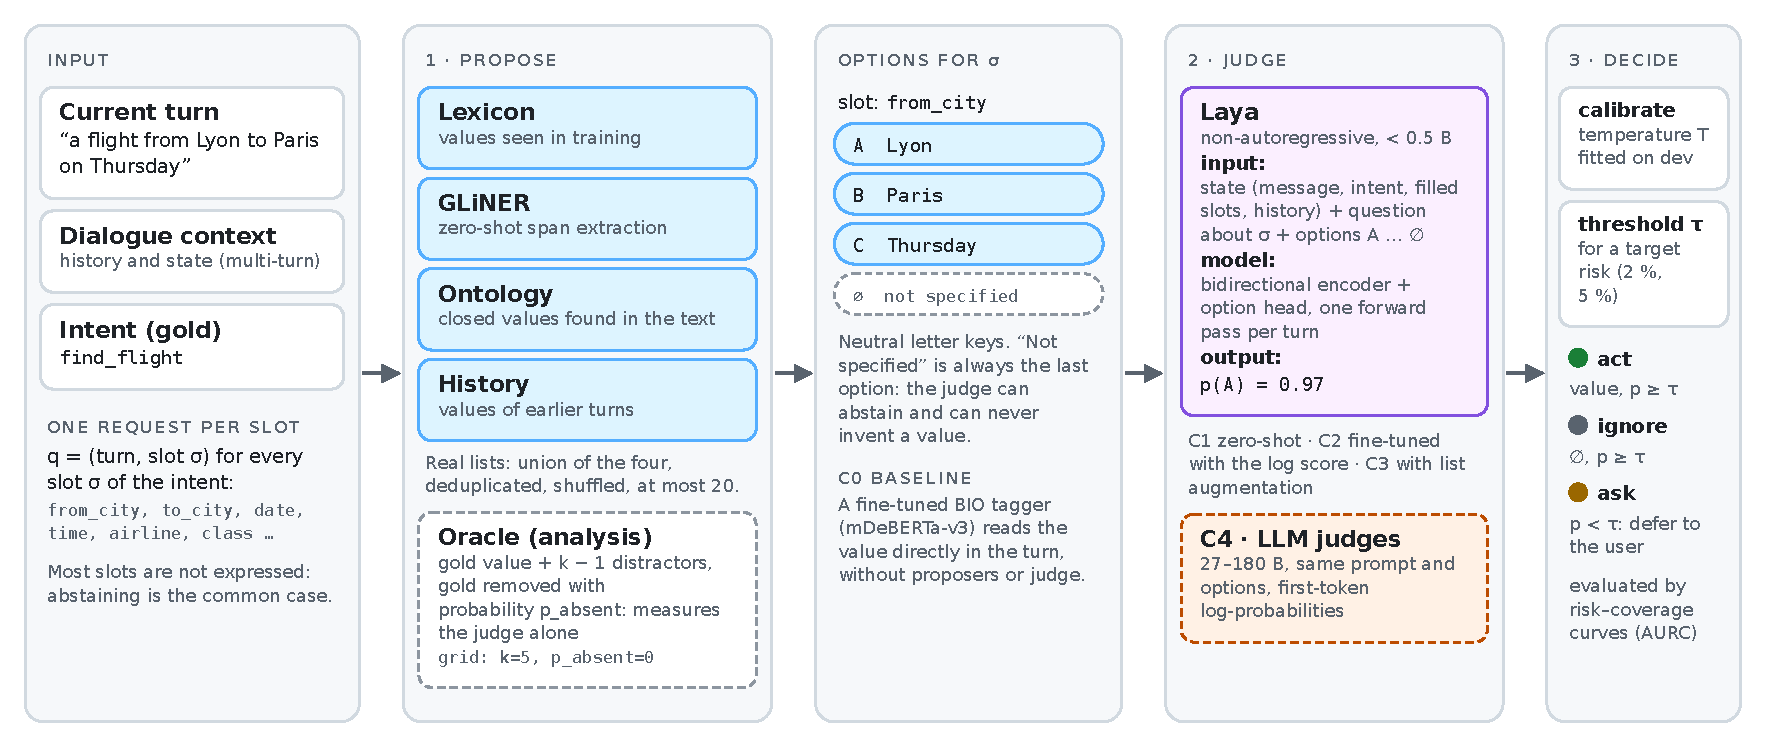
\includegraphics[width=\textwidth]{figures/architecture.pdf}
\caption{The proposer--judge architecture, illustrated on one request: the slot \texttt{from\_city} of the turn ``a flight from Lyon to Paris on Thursday''. \textbf{Input}: one request is issued for every slot of the gold intent, and most of these slots are not expressed. \textbf{1~Propose}: four inexpensive proposers (lexicon of training values, GLiNER, ontology, dialogue history) build the real candidate list; for analysis, an oracle builds a list around the gold value with $k-1$ distractors and removes the gold value with probability $p_{\text{absent}}$. \textbf{Options}: candidates appear under neutral letter keys, followed by ``not specified'' (\none); the distractor C (\emph{Thursday}) is the value of another slot of the same turn, the typical trap of real lists. \textbf{2~Judge}: Laya reads the dialogue state, the question about the slot and the options, and returns a probability per option in one forward pass (C1 zero-shot, C2 fine-tuned, C3 fine-tuned with option-list augmentation); in C4, an LLM judge is scored on the same options. \textbf{3~Decide}: after temperature scaling fitted on development data, a threshold $\tau$ set for a target risk maps the answer to \emph{act} (fill the slot), \emph{ignore} (leave it empty) or \emph{ask} (defer to the user). C0, a fine-tuned BIO tagger, is the classical alternative that reads values directly in the turn, without proposers or judge.}
\label{fig:architecture}
\end{figure}

An \emph{example} $x$ is a user turn: the current utterance $u$, the preceding dialogue history $h$ (empty for single-turn datasets), the current intent or domain $\iota$, and, in multi-turn dialogue, the slots already filled before the turn, $s^{-}$. The schema gives, for each intent $\iota$, the set $\mathcal{S}(\iota)$ of slots that it allows; each slot $\sigma$ has a name and a short natural-language description (\cref{app:conversion}). The gold annotation assigns to each slot either a set of values $V^{*}(x,\sigma)$ expressed in the turn, or nothing.

\Cref{fig:architecture} gives an overview of the architecture on a concrete request; this section formalises it. For every slot $\sigma \in \mathcal{S}(\iota)$ we issue one \emph{request} $q=(x,\sigma)$. A set of proposers $G_1,\dots,G_m$ produces a candidate list
\begin{equation}
  \Cand(q) = \operatorname{dedup}\bigl(G_1(q) \cup \dots \cup G_m(q)\bigr) = (c_1,\dots,c_k), \qquad k \le K,
\end{equation}
where values are normalised before deduplication (\cref{app:conversion}) and the first generator wins ties. A judge $J$ maps the request and its list to a probability distribution over the $k$ candidates and an extra option $\none$ (``not specified''):
\begin{equation}
  p(\cdot \mid q) = J\bigl(x,\sigma,\Cand(q)\bigr) \in \Delta^{k}, \qquad
  \hat{y}(q) = \arg\max_{y \in \Cand(q)\cup\{\none\}} p(y \mid q), \qquad
  \hat{c}(q) = \max_{y} p(y \mid q).
\end{equation}
The predicted value is $\hat{y}(q)$ unless $\hat{y}(q)=\none$, in which case the slot stays empty. An empty list yields $\none$ without calling the judge. The correct option is
\begin{equation}
  y^{*}(q) =
  \begin{cases}
    c_i & \text{if } V^{*}(x,\sigma) \neq \emptyset \text{ and } c_i \in V^{*}(x,\sigma),\\
    \none & \text{otherwise (slot not expressed, or gold value absent from the list).}
  \end{cases}
\end{equation}
Two properties follow directly. The judge cannot output a value that was not proposed, so it cannot hallucinate. And every error falls into exactly one of three classes, which we measure separately (\cref{fig:decomposition,sec:metrics}): a \emph{recall} error (the gold value is not in $\Cand(q)$), a \emph{choice} error (it is in the list but another option is chosen, possibly $\none$), or a \emph{false positive} (a value is chosen for a slot the user did not express).

\begin{figure}[pos=t]
\centering
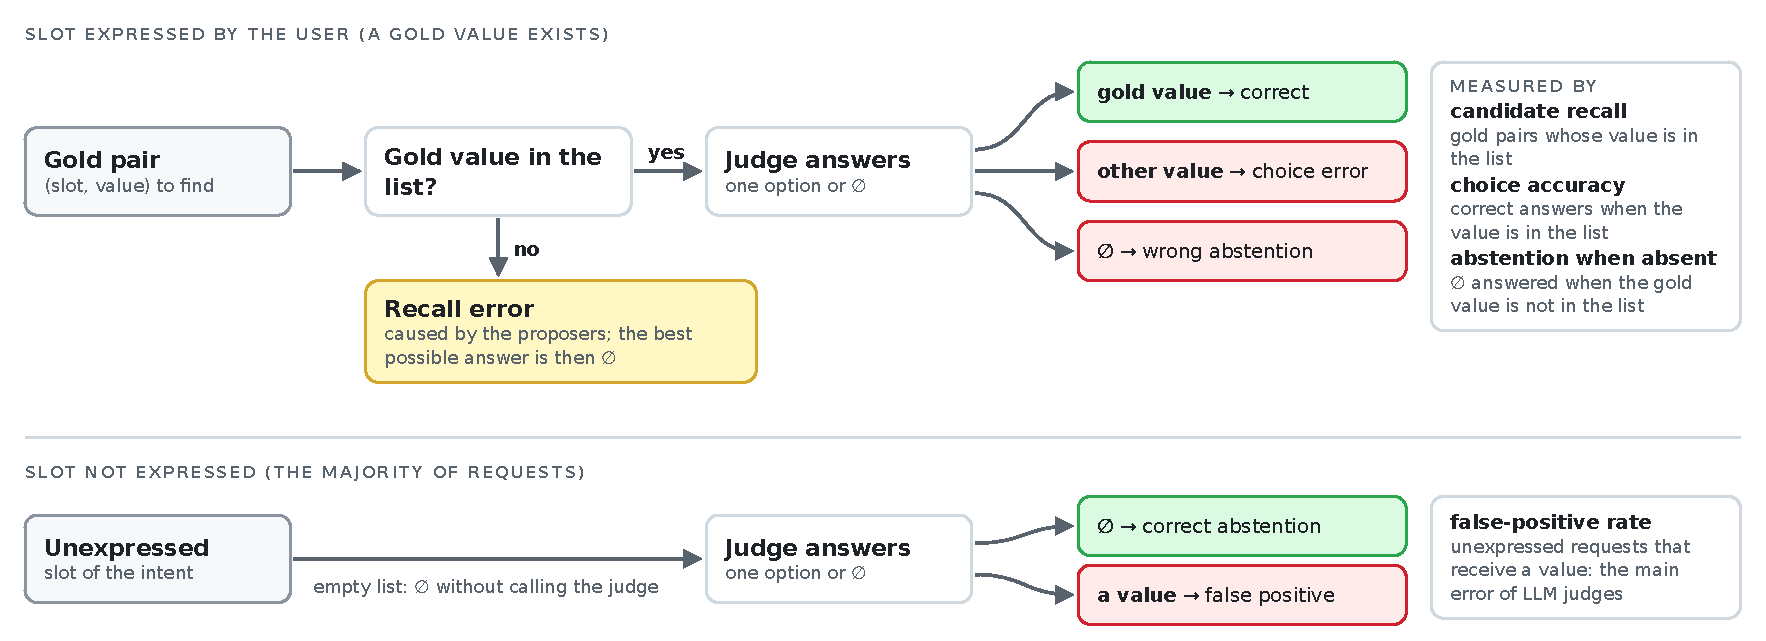
\includegraphics[width=\textwidth]{figures/decomposition.pdf}
\caption{Error decomposition: each request ends in exactly one outcome. \textbf{Top}, a slot expressed by the user: either the gold value is missing from the list, a \emph{recall} error of the proposers for which abstaining is the best possible answer, or it is present and the judge chooses it (correct), chooses another value (\emph{choice} error) or abstains wrongly. \textbf{Bottom}, an unexpressed slot, the majority of requests: the judge must answer \none, and any value is a \emph{false positive}; an empty list is answered \none\ without calling the judge. The measures on the right separate the proposers (candidate recall) from the judge (choice accuracy, abstention when the gold value is absent, false-positive rate).}
\label{fig:decomposition}
\end{figure}

\subsection{The Laya judge}
\label{sec:laya}

Laya \citep{laya2026} is a non-autoregressive decision model released under the Apache-2.0 licence. It encodes a structured \emph{state} (a dictionary of text fields) together with one or more \emph{questions}; each question has typed options rendered as ``\texttt{key: description}'', and a head attached to marker tokens returns a probability distribution over the options of each question in a single forward pass. We use the \texttt{multilingual} checkpoint, built on mmBERT-base \citep{marone2026mmbert} (the English checkpoint is built on ModernBERT-large \citep{warner2025modernbert}), with the runtime pinned to version 0.3.22 and the checkpoint to revision \texttt{7b928d8}. Its encoder accounts for 322\,M parameters for the multilingual checkpoint (mmBERT-base; 421\,M for the English one, according to the model cards), hence ``fewer than half a billion'' parameters in total.

\paragraph{State} The state sent to Laya contains, in this order (Laya truncates a state from the right): the last user message (at most 1,000 characters), the current intent (or domain), the slots already filled (multi-turn only) and the last four turns of history (at most 1,500 characters, truncated from the left).

\paragraph{Question} In the main \emph{single} mode, each request becomes one multiple-choice question whose instruction reads
\begin{quote}\small
\texttt{Which value does the user's last message give for the slot "\{slot\}" (\{description\})?}
\end{quote}
with the candidates as options under neutral letter keys (A, B, \ldots) and a last option ``\texttt{not specified: the last message gives no value for this slot}''. Candidates are shuffled with a seed that depends only on the run seed, the example and the slot, because Laya, like LLM judges \citep{wang2024fair}, has a strong position bias. At most 15 candidates are shown during training and up to 20 during evaluation (\cref{app:hyper}). A \emph{two-step} mode, which first asks whether the slot is expressed and then which candidate is correct, is implemented (\cref{app:prompts}), but its fine-tuned version was not evaluated in this study (hypothesis H4 remains open). All questions of the requests that share a state (same example, intent and filled slots) are grouped into one forward pass: one Laya call per turn.

\subsection{Candidate generation}
\label{sec:candidates}

\paragraph{Oracle candidates} To measure the judge alone, the oracle generator returns the gold value plus $k-1$ distractors, and removes the gold value with probability $p_{\text{absent}}$ when the slot is expressed. Distractors are drawn by a sampler that mixes several strategies, each with a weight: values of the same slot seen in training (\texttt{train\_values}), closed values of the ontology, values of \emph{other} slots of the same utterance (\texttt{other\_slots}), content $n$-grams of the utterance ($n\le 3$), and values from the dialogue state or history. Within a strategy, a value is drawn with probability proportional to $\exp(\mathrm{sim}/0.1)$, where $\mathrm{sim}$ is the character-trigram similarity with the gold value, which yields \emph{hard} distractors. Our main preset, \texttt{hard\_no\_overlap}, additionally excludes boundary variants, i.e.\ values that contain the gold value or are contained in it as whole words (``on april'' or ``april 1'' for ``april''): choosing such a variant is a segmentation error rather than an understanding error, and with real candidates such variants appear naturally when a generator segments badly. The \texttt{hard} preset keeps them and serves as an ablation; the \texttt{easy} preset draws uniformly among all known values of all slots; the \texttt{confusion} preset (used for augmentation, \cref{sec:augmentation}) puts a weight of 3 on \texttt{other\_slots}. Candidates are ``blind'' (no score, source or offsets), so that a judge cannot recognise the gold value from metadata. Three independent random streams, all derived from (seed, example, slot), decide the removal of the gold value, the sequence of distractors and the final order. Lists for $k$ are therefore prefixes of lists for $k+1$, and examples without gold value are nested when $p_{\text{absent}}$ grows, so that sweeps over $k$ and $p_{\text{absent}}$ compare paired conditions.

\paragraph{Real candidates} To measure the whole pipeline, we use the union of four generators, in this priority order: (i) a \emph{lexicon} of the normalised values seen in training for the slot, matched against the $n$-grams of the utterance; (ii) GLiNER \citep{zaratiana2024gliner} (\texttt{urchade/gliner\_multi-v2.1}), zero-shot, with the slot description as label and a threshold of 0.3; (iii) the \emph{ontology}, whose closed values are matched exactly or approximately (similarity $\ge 0.85$) in the utterance; and (iv) the \emph{history} (Multi3WOZ only): the value already in the state, the same attribute in another domain, and known values mentioned in recent turns. The union keeps at most $K=20$ candidates, deduplicated by normalised value, in a shuffled order. The fine-tuned judges are \emph{not} retrained on real candidates: real lists are an out-of-distribution test of the judge trained on oracle lists.

\subsection{Fine-tuning by the log score}
\label{sec:finetuning}

\paragraph{Objective} The released Laya package does not include its training module; the original model was trained with policy-gradient rewards derived from strictly proper scoring rules \citep{laya2026}. We fine-tune it with direct supervision instead: the loss of a question with options $o_1,\dots,o_n$ and correct option $o_{t}$ is the log score $-\log p(o_{t})$ \citep{gneiting2007scoring}, i.e.\ the cross-entropy over its options. This is the same family of strictly proper rules, optimised by supervised learning rather than by reinforcement. We reimplemented the training loop on top of Laya's inference primitives (state encoding, collation and decision head), so that the encoding of a question at training time is exactly the one used for prediction, and we save checkpoints in Laya's own format.

\paragraph{Items built by the inference code} Every training request goes through the function that prepares Laya's questions at evaluation time: same state, same instruction templates, same shuffled order, same truncation of the candidate list. Only the target is added: the position of the gold value among the options, or the ``not specified'' option when the slot is not expressed or the gold value is not in the list. A format mismatch between training and evaluation is therefore impossible by construction. Training requests are built on the training split with the evaluation's request builder (all slots allowed by the gold intent, \cref{sec:setup}).

\paragraph{Class imbalance} Most requests concern slots that the user did not express (about 94\% on MultiATIS++). We keep all requests with an expressed slot and at most two unexpressed requests per expressed request in each example (\texttt{unexpressed\_ratio} $=2$), drawn with the run seed; this gives 43,000 to 189,000 training questions per dataset and language (\cref{tab:trainsizes}). On MultiATIS++ English this yields 43,007 training questions from 4,478 training utterances.

\paragraph{Optimisation and checkpoint selection} We train for three epochs with AdamW (learning rates $2\times10^{-5}$ for the encoder and $10^{-4}$ for the head), a linear warm-up over 5\% of the steps followed by cosine decay, batches of 32 questions, gradient clipping at 1.0, bf16 autocast over fp32 weights and gradient checkpointing (\cref{tab:hyper}). After each epoch we evaluate the slot F1 on all requests of the first 300 development examples (same distribution as at test time) and keep the best epoch. We first selected on the development loss, but the loss is distorted by over-confidence: one C3 seed kept an epoch whose loss was lower but whose decisions were worse; selecting on development F1 removed this failure mode (\cref{sec:threats}). Checkpoints are saved with neutral temperatures ($T=1$); calibration is a separate, post-hoc step (\cref{sec:decision}).

\paragraph{Bilingual training} For the joint English--French condition, the items of both languages are concatenated; each language keeps its own ontology (slot descriptions in that language where available) and its own oracle candidates fitted on its own training split. The checkpoint is selected on the English development set, with oracle candidates. The main configuration uses \emph{monolingual} models (one per dataset and language); bilingual training and English-to-French transfer are analysed in \cref{sec:rq3}, where bilingual training turns out to be unstable with real candidates.

\subsection{Option-list augmentation}
\label{sec:augmentation}

A judge trained on a single list shape (oracle, $k=5$, gold always present) may fail when the context changes: longer lists, a missing gold value, other kinds of distractors. Our augmentation draws, for each training example, one combination of list size, missing-value rate and distractor preset, uniformly among the Cartesian product of the following lists (the order of options is already shuffled by the judge):
\begin{itemize}
  \item \textbf{C3 v1} (generic): $k\in\{2,5,10,20\}$, $p_{\text{absent}}\in\{0, 0.2, 0.5\}$, distractors $\in\{\texttt{easy},\texttt{hard\_no\_overlap}\}$;
  \item \textbf{C3 v2} (confusion-oriented): $k\in\{2,2,3,3,5,10,20\}$ (short lists twice as likely), $p_{\text{absent}}\in\{0, 0.2, 0.5\}$, distractors $\in\{\texttt{confusion},\texttt{hard\_no\_overlap}\}$.
\end{itemize}
Version~2 was designed after analysing the failure of version~1 on real candidates (\cref{sec:rq5}): real lists are short and their main trap is a value of \emph{another slot} of the same utterance (``boston'' proposed as the stop-over city when it is the departure city), whereas the \texttt{easy} distractors of version~1 are of other types and easy to reject. On 200 training examples, 63\% of the distractors for unexpressed slots come from other slots of the utterance with \texttt{confusion}, against 33\% with \texttt{hard\_no\_overlap}. In the remainder of the paper ``C3'' denotes version~2; version~1 is kept as an ablation of the augmentation design. Note that with the judge's default of 15 options at training time, $k=20$ is truncated to 15 (\cref{app:hyper}).

\subsection{Calibrated three-zone decision}
\label{sec:decision}

\paragraph{Calibration} The unit is a judged request: the judge's distribution over its options and the correct option $y^{*}$. Requests with an empty list are excluded, since their decision ($\none$) is certain and identical for all judges. We fit on development data (i) \emph{temperature scaling} \citep{guo2017calibration}, $p_T(y) \propto p(y)^{1/T}$ with $T$ minimising the negative log-likelihood (NLL), which preserves the ranking of options and hence the decision, and (ii) \emph{isotonic regression} \citep{zadrozny2002transforming} of the correctness of the selected option on its confidence. We report NLL, the multi-class Brier score and the expected calibration error (ECE, 15 equal-width bins).

\paragraph{Decision} For a confidence $\hat c$ and a threshold $\tau$, the policy is
\begin{equation}
  \text{decision}(q) =
  \begin{cases}
    \textsc{act} \ (\text{fill } \hat y) & \text{if } \hat c \ge \tau \text{ and } \hat y \neq \none,\\
    \textsc{ignore} \ (\text{leave empty}) & \text{if } \hat c \ge \tau \text{ and } \hat y = \none,\\
    \textsc{ask} \ (\text{defer to the user or a costlier judge}) & \text{if } \hat c < \tau.
  \end{cases}
\end{equation}
\emph{Coverage} is the share of requests decided without asking and \emph{risk} the error rate among them \citep{geifman2017selective}. Sweeping $\tau$ over all observed confidences (ties treated together) gives the risk--coverage curve, whose area (AURC; lower is better) summarises how well the confidences rank the errors. For a target risk (2\% and 5\% in the main grid), the threshold that maximises coverage is chosen on development data and then applied unchanged. As long as the test set is closed, we split the development set into two halves of clusters (dialogues or utterances), fit on one half, evaluate on the other, in both directions, and average (two folds). For the test-set results (\cref{sec:rq4}), calibration and thresholds are fitted on the whole development set and applied once, unchanged, to the test set.

\subsection{LLM judges}
\label{sec:llmjudge}

The LLM judges play exactly the same role. Each request is rendered with a fixed, versioned prompt (\texttt{slot-judge-v1}, reproduced in \cref{app:prompts}) that contains the slot, its description, the intent, the filled slots, the last four turns of history, the last user message with its language, and the candidates under letter keys followed by a ``not specified'' option, in the same shuffled order as for Laya. The model is asked to answer with a single letter. We generate one token at temperature 0 and read the top-20 log-probabilities of that first token; the probabilities of all tokenisations of a letter (``A'', ``\textvisiblespace A''\ldots) are summed and renormalised over the letters offered. If no letter appears in the top-20, the distribution is uniform and the case is logged (this never occurred in our checks, \cref{sec:llms}). Reasoning (``thinking'') is switched off through the chat template, which we verified per model family. This logit-based reading gives the LLM a full probability distribution over the same options as Laya, which is required for a fair calibration comparison.

%% ===========================================================================
\section{Experimental setup}
\label{sec:setup}
%% ===========================================================================

\begin{figure}[pos=t]
\centering
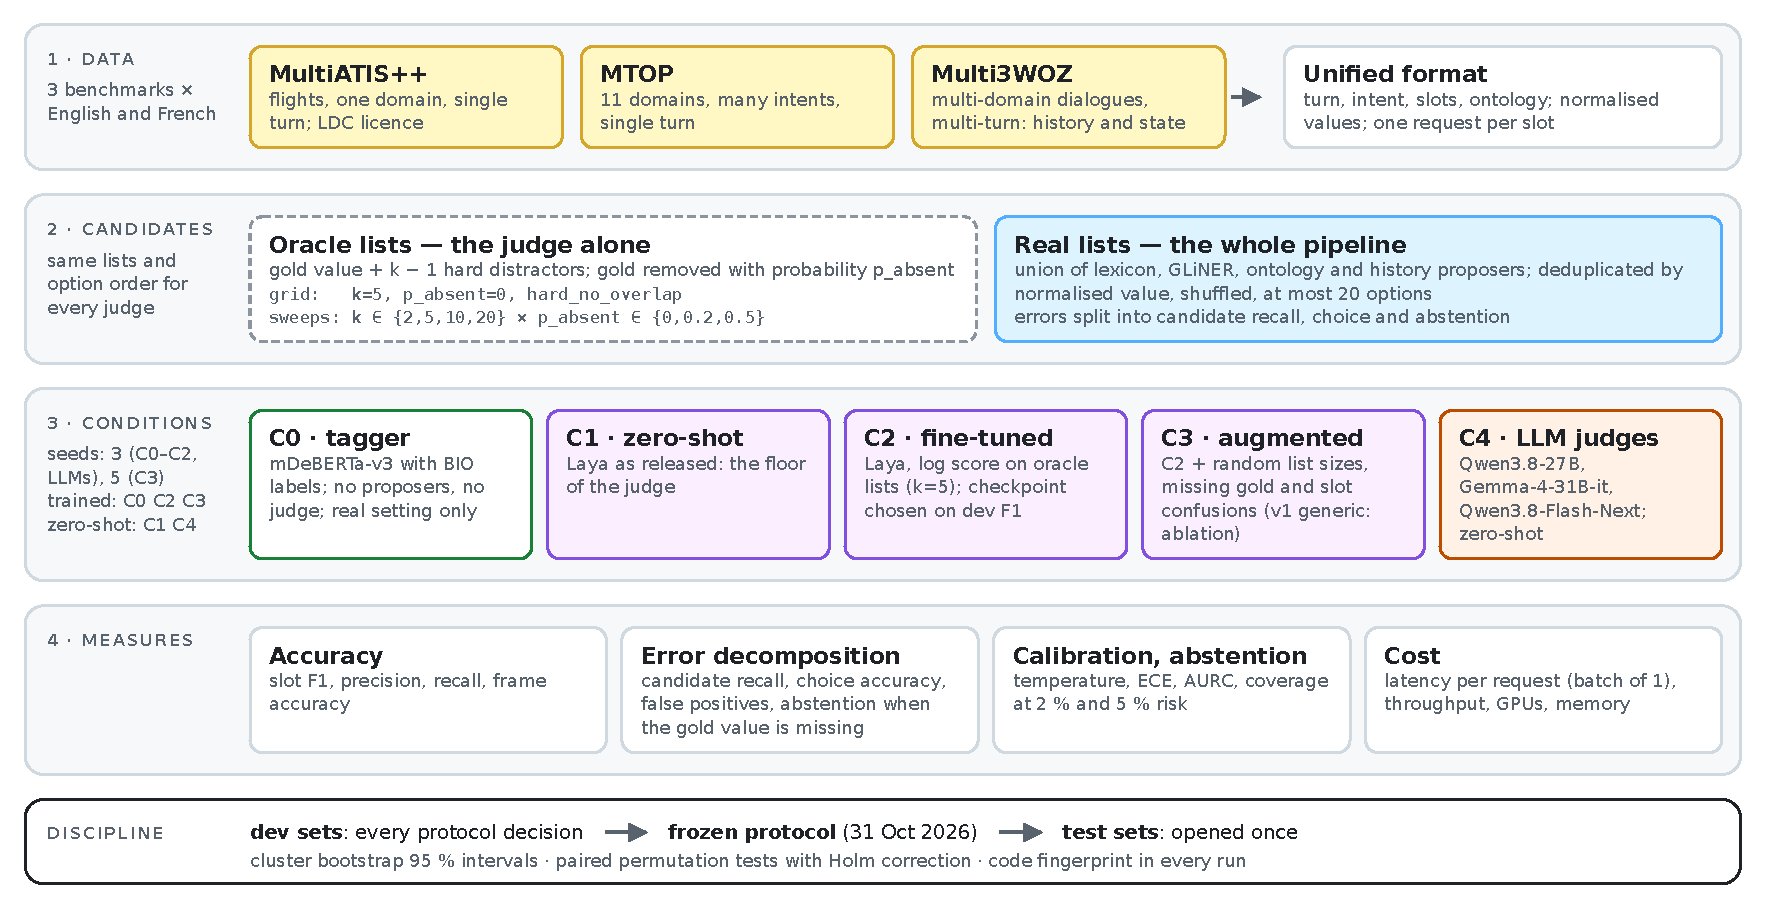
\includegraphics[width=\textwidth]{figures/protocol.pdf}
\caption{Experimental protocol. \textbf{(1)} Three span-annotated benchmarks, each in English and French, are converted to a unified format with one request per slot of the gold intent. \textbf{(2)} Every judge sees the same candidate lists in the same order: oracle lists isolate the judge (grid setting, and sweeps over the list size $k$ and the missing-gold rate $p_{\text{absent}}$), real lists from four proposers measure the whole pipeline. \textbf{(3)} Five conditions: a fine-tuned BIO tagger (C0), Laya zero-shot (C1), fine-tuned (C2) and fine-tuned with option-list augmentation (C3), and three open-weight LLM judges (C4). \textbf{(4)} Four families of measures: accuracy, error decomposition, calibration and selective decision, and cost. All protocol decisions were taken on development sets; the protocol was then frozen and each test set opened once.}
\label{fig:protocol}
\end{figure}

\subsection{Datasets and conversion}
\label{sec:datasets}

\Cref{fig:protocol} summarises the experimental design: the data, the two kinds of candidate lists, the compared conditions, the measures, and the separation between development and test data. The following subsections detail each part.

All three benchmarks annotate slots as text spans; we convert them to the candidate-selection format of \cref{sec:formulation} with a common schema and deterministic value normalisation (case, Unicode, numbers written in words, times, \cref{app:conversion}). Each converted split is written with a manifest that records the SHA-256 of the raw and produced files. \Cref{tab:datasets} summarises the data.

\begin{table}[pos=t]
\centering
\small
\caption{Datasets after conversion. Split sizes in utterances (MultiATIS++, MTOP) or dialogues (Multi3WOZ, one example per user turn). Request volumes are the number of (example, slot) requests submitted to the judge on the development split.}
\label{tab:datasets}
\begin{tabular}{@{}lllp{3.0cm}p{4.2cm}@{}}
\toprule
Dataset & Lang. & Turns & Train / dev / test & Dev requests \\
\midrule
MultiATIS++ & EN, FR & single & 4,478 / 500 / 893$^{a}$ & 30,310 per language (1,682 EN / 1,678 FR gold pairs) \\
MTOP & EN & single & 15,667 / 2,235 / 4,386 & 15,096 \\
     & FR & single & 11,814 / 1,577 / 3,193 & 9,832 \\
Multi3WOZ & EN, FR & multi & 7,440 / 860 / 860 dial. & 68,863 per language (7,708 gold pairs) \\
\bottomrule
\end{tabular}

\smallskip
\footnotesize $^{a}$ The LDC release provides only train (4,978) and test (893); we draw the development set from the training set (the 500 identifiers with the smallest SHA-256), aligned across languages. This is not the 4,488/490 split of the original paper.
\end{table}

\paragraph{MultiATIS++} \citep{xu2020multiatis,mansour2021atis7}: flight-information requests, one domain, with BIO labels. Spans are recovered as character offsets; for the rare multi-intent utterances (1--2\%), the first intent is the main intent. Slot descriptions were written once by hand (``fromloc.city\_name'' $\rightarrow$ ``departure city''), in English for English and in French for French, and frozen before evaluation. Thirteen lines of the French training split whose number of labels differs from the number of tokens are skipped.

\paragraph{MTOP} \citep{li2021mtop}: eleven domains and many intents (113 intents and 75 slots in English, 110 intents and 73 slots in French). We keep top-level slots; a nested slot becomes one top-level slot whose value is the full covered text, and its sub-tree is kept for a separate analysis. Slot descriptions were written by hand in English and used for both languages.

\paragraph{Multi3WOZ} \citep{hu2023multi3woz}: culturally adapted, multi-parallel versions of MultiWOZ dialogues, corrected release of 15 December 2023. One example is one user turn; its slots are the \emph{difference} between the dialogue state after and before the turn, the definition consistent with joint goal accuracy. We keep the five usual domains (hotel, train, restaurant, attraction, taxi; 30 slots). The history and the state before the turn are given to the judges. Multi3WOZ has no per-turn intent; we therefore query only the slots of the gold domain of the turn (\emph{domain filter}), which plays the role of the gold intent in the other datasets, and we pass the domain to the judge as a hint. Turns without a domain (15\%) are queried on all 30 slots. On 300 development turns, the filter reduces the number of requests from about 30 to 11 per turn, of which 12.6\% are expressed, and leaves out 8 of 420 gold pairs (1.9\%) that belong to another domain, which caps recall. The alternative of querying all 30 slots at every turn would quadruple the requests, 99\% of them unexpressed.

\paragraph{Requests} In all datasets, the judge receives the gold intent (or domain) and is asked about every slot that this intent allows. This isolates slot filling from intent classification; end-to-end evaluation with predicted intents is left for future work. About 94\% of the requests concern slots that are not expressed on MultiATIS++, which makes abstention a central part of the task.

\subsection{Conditions}
\label{sec:conditions}

\begin{table}[pos=t]
\centering
\small
\caption{Compared conditions. All judges see the same candidate lists and the same option order for a given seed.}
\label{tab:conditions}
\begin{tabular}{@{}lp{6.3cm}p{5.0cm}@{}}
\toprule
Code & Condition & Role \\
\midrule
C0 & Sequence tagger alone (mDeBERTa-v3-base, BIO labelling, fine-tuned) & classical extraction baseline (real setting only) \\
C1 & Laya zero-shot (published \texttt{multilingual} checkpoint) & floor of the judge \\
C2 & Laya fine-tuned, oracle lists $k=5$, $p_{\text{absent}}=0$ & effect of fine-tuning \\
C3 & Laya fine-tuned with confusion-oriented augmentation (v2) & robustness to list shape (RQ5) \\
C3 v1 & Laya fine-tuned with generic augmentation & ablation of the augmentation design \\
C4 & Open-weight LLM judges (three models), zero-shot & reference for the same role \\
\bottomrule
\end{tabular}
\end{table}

\Cref{tab:conditions} lists the conditions. Each judge is evaluated with oracle candidates (\texttt{hard\_no\_overlap}, $k=5$, $p_{\text{absent}}=0$: the \emph{grid setting}) and with real candidates. Sweeps over $k\in\{2,5,10,20\}$ and $p_{\text{absent}}\in\{0,0.2,0.5\}$, the \texttt{hard} distractor preset and the English-to-French transfer are analyses, run for the Laya judges on MultiATIS++ English. Few-shot LLM judges, a generative LLM extractor without proposers, the two-step judge mode (\cref{app:prompts}), unseen-domain splits and schema perturbations are left for future work (\cref{sec:limitations}).

\paragraph{The sequence tagger (C0)} C0 is the classical alternative to the proposer--judge architecture: a multilingual encoder, \texttt{microsoft/mdeberta-v3-base} (278\,M parameters; revision \texttt{a048466}, weights from the safetensors conversion \texttt{refs/pr/5}), fine-tuned to label every word of the current utterance with a BIO tag of the slots of the ontology (\texttt{B-}$\sigma$ for the first word of a value of slot $\sigma$, \texttt{I-}$\sigma$ for the following words of that value, \texttt{O} outside any value; in ``from New York to Paris'', \emph{New} is \texttt{B-from\_city}, \emph{York} is \texttt{I-from\_city} and \emph{Paris} is \texttt{B-to\_city}), in the spirit of JointBERT \citep{chen2019jointbert} but without an intent head (the gold intent is given to all conditions). Words are those of the candidate generators, and the label of a word is read on its first sub-word. Training labels come from the gold spans of the current utterance only, so that values taken from the history, the dialogue context or canonical forms that do not occur in the text cannot be learnt. The model is trained for 10 epochs with AdamW (learning rate $3\times10^{-5}$, batch 32, linear warm-up over 10\% of the steps), with three seeds, and the epoch with the best span F1 on the development set is kept. At inference, the decoded spans are normalised like the gold values; the best-scoring span of a slot is its only candidate, and C0 fills the slot with it, or answers ``not specified'' when the tagger proposes nothing. C0 therefore has no oracle setting.

\subsection{LLM judges and their configuration}
\label{sec:llms}

We selected recent open-weight models that fit the hardware and cover two families and two architectures (\cref{tab:llms}). All are served offline by vLLM~0.30.0 in text-only mode, with a context of 4,096 tokens, greedy decoding of one token and reasoning disabled. On 20 development examples (940 requests), the three models never produced a first token without an option letter. A fourth model from a third family, Mistral-Small-4-119B, could not be loaded by vLLM~0.30.0 (its text configuration declares no architecture) and was withdrawn; it may be added with a later vLLM version. A preliminary model (Qwen3-32B) used during development is not reported in the main results. The LLM judges are served with vLLM \citep{kwon2023vllm}, version 0.30.0.

\begin{table}[pos=t]
\centering
\small
\caption{Judges. Revisions are Hugging Face commit hashes (abbreviated); all are recorded in \texttt{MODELES.lock.json}.}
\label{tab:llms}
\resizebox{\textwidth}{!}{%
\begin{tabular}{@{}llllll@{}}
\toprule
Judge & Architecture & Parameters & Precision & GPUs & Revision \\
\midrule
Laya \texttt{multilingual} \citep{laya2026} & encoder, non-autoregressive & 0.32\,B (encoder) & fp32 (bf16 autocast) & 1 (shared) & \texttt{7b928d8} \\
Qwen3.8-27B \citep{qwen38} & dense decoder & 27.8\,B & BF16 & 1 & \texttt{1d4bf0f} \\
Gemma-4-31B-it \citep{gemma4report} & dense decoder & 31.3\,B & BF16 & 1 & \texttt{842da37} \\
Qwen3.8-Flash-Next-FP8 \citep{qwen38flashnext} & MoE (10 of 512 experts active) & 180\,B & FP8 & 2 & \texttt{236dfdf} \\
\bottomrule
\end{tabular}}
\end{table}

\subsection{Metrics}
\label{sec:metrics}

\paragraph{Accuracy} The main metric is the micro-averaged F1 over (slot, value) pairs, a ``not specified'' prediction not counting as a prediction, with precision and recall. \emph{Frame accuracy} is the share of examples whose whole set of slots is exactly right, with no extra slot; it makes the cost of false positives visible. Joint goal accuracy, the official Multi3WOZ metric, is not reported: our requests are restricted to the gold domain and evaluated turn by turn, which does not match the cumulative dialogue state it scores.

\paragraph{Decomposition} Because the F1 is dominated by abstention when most slots are unexpressed, we always report side by side: \emph{candidate recall} (share of gold pairs whose value is in the list), \emph{choice accuracy given present} (share of gold pairs correctly chosen when the value is in the list: the judge alone), the \emph{false-positive rate} (share of unexpressed requests for which a value is chosen), and the \emph{abstention rate when the gold value is absent} (share of requests with an expressed slot but no gold value in the list that are answered ``not specified'', the only answer that does not create an error).

\paragraph{Calibration and abstention} NLL, Brier score, ECE, temperature $T$, AURC, and coverage at 1\%, 2\% and 5\% risk (\cref{sec:decision}).

\paragraph{Cost} Latency per request (p50 and p95), throughput (requests per second), number of GPUs and memory. Accuracy runs are batched (Laya batches of 128 states, LLM batches of 256 prompts), and their latencies are batch-amortised. Latency proper is measured in separate runs with batches of size one (one request per call to the judge), on the first 100 development examples of each English dataset with oracle lists in the grid setting, seed 13, with nothing else running on the GPUs. For Laya, the first occurrence of each input length costs about 80\,ms, once (kernel selection for a new tensor shape); we report the p95 latency after this warm-up as well, since a deployed system would pad inputs to a few fixed lengths.

\subsection{Statistical protocol}
\label{sec:stats}

\paragraph{Seeds} Fine-tuned conditions use three seeds (C0, C2) or five (C3); the seed controls the training order, the subsampling of unexpressed requests and the oracle candidate draws. LLM judges are deterministic; their seeds only change the candidate draws (three in the final grid, one in the current development runs).

\paragraph{Intervals and tests} Confidence intervals (95\%) are percentile bootstrap intervals with 1,000 resamples of \emph{clusters} (dialogues for Multi3WOZ, utterances otherwise), never of isolated turns or requests. Each cluster is summarised by additive counts, and every metric is a ratio of sums with the same definitions as the point estimates. Paired comparisons use the clusters common to both systems: the difference and its interval come from a paired bootstrap, and the $p$-value from a permutation test that swaps the two systems cluster by cluster (10,000 permutations, two-sided). The Holm correction is applied over all comparisons and metrics of a family (stated with each result). With 10,000 permutations the smallest attainable $p$-value is $1/10{,}001$, so the smallest Holm-corrected value depends on the family size; we report such floor values as ``$p<10^{-4}$ before correction''.

\paragraph{Development and test discipline} All protocol decisions (distractor preset, checkpoint criterion, augmentation version, monolingual versus bilingual training, decision thresholds) were taken on development data. The protocol of the final runs (grid, seeds, analyses, families of tests, decision procedure) was then written down and frozen on 31 October 2026, together with the fingerprint of the code (\texttt{docs/protocole\_test.md} in the repository), and each test set was used in a single pass, from 31 October to 1 November 2026. During the early development phase, the MultiATIS++ English test split was opened several times; results obtained there are used only as exploratory evidence and are flagged as such (\cref{sec:threats}).

\subsection{Hardware, software and reproducibility}
\label{sec:repro}

All runs use one machine with two NVIDIA H200 NVL GPUs (143,771\,MiB each, driver 595.71.05, CUDA 13.0 runtime from Python wheels). Laya fits on a fraction of one GPU (peak memory 1.7\,GiB); the LLMs take one GPU (27--31\,B) or both (180\,B). The environment is locked with \texttt{uv} (Python 3.12.15, PyTorch 2.13.0, transformers 5.16.1, vLLM 0.30.0, laya 0.3.22, GLiNER 0.2.29); model revisions are pinned and runs are executed offline. Every run writes its resolved configuration, its predictions (one line per request, with the full probability vector) and its metrics, together with the hash of the configuration, the SHA-256 of the data manifests, and a fingerprint of all source and configuration files (\texttt{code\_sha256}), which does not depend on the version-control metadata of the machine. Reruns with the same seed give identical metrics, and repeated trainings give the same losses to the third decimal. \Cref{app:hyper} lists all hyperparameters.

%% ===========================================================================
\section{Results}
\label{sec:results}
%% ===========================================================================

All results in this section are \textbf{test-set results} of the frozen protocol (\cref{sec:stats}), obtained in a single pass after every decision had been taken on development data. Unless stated otherwise, values are means over seeds (three for C0, C1, C2 and the LLM judges, five for C3) with the standard deviation across seeds; seed-to-seed standard deviations of the slot F1 are at most 0.012 for every judge in the main grid. The main configuration uses monolingual models (one per dataset and language); bilingual training is analysed in \cref{sec:rq3}. Paired comparisons use seed 13 against seed 13, cluster permutation tests and the Holm correction within the three families of the protocol: C2 against each LLM judge (108 tests), C3 against C2 (36 tests), and C0 against the best Laya judge chosen on development data (18 tests). Latencies were measured on development examples (\cref{sec:metrics}). The per-run metrics, intervals and comparison tables are in the code repository.

%% ---------------------------------------------------------------------------
\subsection{RQ1: accuracy and cost against LLM judges}
\label{sec:rq1}
%% ---------------------------------------------------------------------------

\paragraph{A small fine-tuned judge is far more accurate} \Cref{tab:rq1-atis} compares the judges on MultiATIS++ English. Zero-shot, Laya is not a usable slot judge: its F1 is 0.025 in the grid setting and 0.275 with real candidates, it fills 83\% of the unexpressed slots with oracle lists, and its choice accuracy given a present gold value is only 0.20: the information is missing from the model, not from the decision rule. After fine-tuning, it reaches an F1 of 0.941 with oracle candidates and 0.828 with real ones. The three LLM judges stay between 0.36 and 0.43 (oracle) and 0.52 and 0.53 (real).

\begin{table}[pos=t]
\centering
\small
\caption{MultiATIS++ English, test set: fine-tuned Laya against three open-weight LLM judges. Oracle: \texttt{hard\_no\_overlap}, $k=5$, $p_{\text{absent}}=0$. Mean $\pm$ s.d.\ over seeds (C2 and LLMs: 3; C3: 5). ``Choice'' = choice accuracy given that the gold value is in the list; FP = false-positive rate on unexpressed slots; frame acc.\ = share of utterances whose whole set of slots is exactly right.}
\label{tab:rq1-atis}
\setlength{\tabcolsep}{4pt}
\begin{tabular}{@{}llcccccc@{}}
\toprule
Cand. & Judge & F1 & P & R & Frame acc. & Choice & FP \\
\midrule
\multirow{5}{*}{oracle}
 & C2 Laya FT & \textbf{0.941} $\pm$ 0.002 & \textbf{0.932} & 0.951 & \textbf{0.785} & 0.956 & \textbf{0.004} \\
 & C3 Laya FT + aug. & 0.935 $\pm$ 0.004 & 0.927 & 0.942 & 0.759 & 0.947 & \textbf{0.004} \\
 & Gemma-4-31B & 0.427 $\pm$ 0.001 & 0.275 & 0.955 & 0.038 & 0.959 & 0.145 \\
 & Qwen3.8-Flash-Next (180\,B) & 0.395 $\pm$ 0.001 & 0.248 & \textbf{0.968} & 0.025 & \textbf{0.973} & 0.169 \\
 & Qwen3.8-27B & 0.361 $\pm$ 0.001 & 0.222 & 0.964 & 0.025 & 0.968 & 0.194 \\
\midrule
\multirow{5}{*}{real}
 & C2 Laya FT & 0.828 $\pm$ 0.002 & \textbf{0.829} & 0.826 & \textbf{0.549} & 0.866 & \textbf{0.004} \\
 & C3 Laya FT + aug. & \textbf{0.829} $\pm$ 0.007 & \textbf{0.829} & 0.830 & 0.542 & 0.870 & 0.005 \\
 & Gemma-4-31B & 0.531 $\pm$ 0.002 & 0.391 & 0.828 & 0.084 & 0.868 & 0.069 \\
 & Qwen3.8-Flash-Next (180\,B) & 0.528 $\pm$ 0.003 & 0.384 & \textbf{0.843} & 0.085 & \textbf{0.884} & 0.072 \\
 & Qwen3.8-27B & 0.522 $\pm$ 0.003 & 0.379 & 0.838 & 0.084 & 0.879 & 0.073 \\
\bottomrule
\end{tabular}
\end{table}

\paragraph{The gap is an abstention gap on MultiATIS++} On this dataset, the LLM judges choose the right value at least as well as the fine-tuned judge when it is in the list (choice accuracy 0.87--0.97, against 0.87--0.96), including the 180\,B mixture-of-experts model: in the 12 paired comparisons of choice accuracy on MultiATIS++ (two languages, two candidate types, three LLMs), the differences range from $-0.022$ to $0.000$, five of them significant in favour of the LLM. The whole difference comes from abstention: the LLM judges fill 15--21\% of the unexpressed slots with oracle lists and 7\% with real lists, against 0.4--0.5\% and 0.4--0.7\% for the fine-tuned judges (C2 and C3). Frame accuracy, which requires all slots of an utterance to be right and no extra one, makes this visible: 0.79 for C2 against at most 0.04 for the LLMs. Size does not solve the problem: the 180\,B model is no better than the 27--31\,B dense models.

\paragraph{The result holds across datasets, languages and families} \Cref{tab:rq1-all} extends the comparison to the three benchmarks in English and French. A fine-tuned judge is the best \emph{judge} in every row (the sequence tagger C0 is discussed in \cref{sec:rq2-tagger}). Of the 108 paired comparisons between C2 and the three LLMs (6 dataset--language pairs $\times$ 2 candidate types $\times$ 3 LLMs $\times$ 3 metrics, Holm), 96 are significant in favour of C2: all 36 on slot F1, all 36 on the false-positive rate, and the 24 on choice accuracy outside MultiATIS++. The F1 gains are $+0.51$ to $+0.59$ on MultiATIS++ with oracle lists and $+0.28$ to $+0.32$ with real lists, $+0.20$ to $+0.25$ and $+0.09$ to $+0.13$ on MTOP, and $+0.10$ to $+0.19$ and $+0.10$ to $+0.14$ on Multi3WOZ. Unlike MultiATIS++, the LLMs also choose less well on MTOP and Multi3WOZ (choice accuracy 0.73--0.89 against 0.83--0.96 for C2; differences $+0.06$ to $+0.18$): MTOP has many intents and slots, and Multi3WOZ requires reading the history and database-like values. Multi3WOZ is the most favourable dataset for the LLMs (false-positive rates of 1.6--2.6\%, thanks to the domain filter), MTOP and MultiATIS++ the least favourable (15--21\% with oracle lists). Among the LLMs, Gemma-4-31B is the best in 11 of the 12 settings.

\begin{table}[pos=t]
\centering
\small
\caption{Slot F1 on the test sets of the three benchmarks (mean over seeds). ``Recall'' is candidate recall of the real lists (1.000 for oracle lists by construction). C0: sequence tagger alone (real setting only; in italics when it beats every judge); C1: zero-shot Laya; C2: fine-tuned Laya; C3: fine-tuned with confusion-oriented augmentation; three seeds except C3 (five). Best judge per row in bold.}
\label{tab:rq1-all}
\setlength{\tabcolsep}{3.5pt}
\begin{tabular}{@{}llllccccccc@{}}
\toprule
Dataset & Lang. & Cand. & Recall & C0 & C1 & C2 & C3 & Qwen3.8-27B & Gemma-4-31B & Flash-Next 180\,B \\
\midrule
MultiATIS++ & EN & oracle & 1.000 & -- & 0.025 & \textbf{0.941} & 0.935 & 0.361 & 0.427 & 0.395 \\
            & EN & real   & 0.959 & \emph{0.949} & 0.275 & 0.828 & \textbf{0.829} & 0.522 & 0.531 & 0.528 \\
            & FR & oracle & 1.000 & -- & 0.025 & \textbf{0.925} & 0.921 & 0.339 & 0.383 & 0.368 \\
            & FR & real   & 0.948 & \emph{0.923} & 0.276 & \textbf{0.832} & 0.828 & 0.525 & 0.539 & 0.556 \\
MTOP & EN & oracle & 1.000 & -- & 0.143 & \textbf{0.953} & 0.951 & 0.704 & 0.753 & 0.727 \\
     & EN & real   & 0.751 & \emph{0.904} & 0.433 & 0.690 & \textbf{0.695} & 0.563 & 0.583 & 0.558 \\
     & FR & oracle & 1.000 & -- & 0.148 & \textbf{0.951} & 0.942 & 0.706 & 0.753 & 0.736 \\
     & FR & real   & 0.675 & \emph{0.833} & 0.335 & 0.625 & \textbf{0.629} & 0.525 & 0.529 & 0.528 \\
Multi3WOZ & EN & oracle & 1.000 & -- & 0.072 & 0.940 & \textbf{0.946} & 0.822 & 0.844 & 0.813 \\
          & EN & real   & 0.888 & 0.733 & 0.196 & \textbf{0.853} & 0.852 & 0.750 & 0.762 & 0.744 \\
          & FR & oracle & 1.000 & -- & 0.056 & 0.917 & \textbf{0.919} & 0.752 & 0.753 & 0.730 \\
          & FR & real   & 0.550 & 0.380 & 0.121 & \textbf{0.592} & 0.588 & 0.459 & 0.474 & 0.458 \\
\bottomrule
\end{tabular}
\end{table}

\paragraph{Cost} \Cref{tab:latency} gives the latency of one request judged alone, measured on development examples. The fine-tuned judge answers in 7.9--8.5\,ms (p50) on a fraction of one GPU, against 24.6--35.1\,ms for Gemma-4-31B, 34.7--50.5\,ms for Qwen3.8-27B and 40.5--49.4\,ms for the 180\,B model on two GPUs: a ratio of 3.1 to 6.0. Once each input length has been seen, its p95 latency stays within 1\,ms of the median (8.0--9.4\,ms); the first occurrence of a length costs about 80\,ms once, which dominates the raw p95 on MTOP and Multi3WOZ, whose 100 examples contain many distinct lengths. With batches, the gap widens: with oracle lists on MultiATIS++, the fine-tuned judge processes 691 requests per second on one GPU, against 83 for the 180\,B model on two GPUs and 38 and 18 for the dense 31\,B and 27\,B models on one GPU (a throughput ratio of 8 to 38); on Multi3WOZ, where the history makes inputs longer, 360--370 requests per second against 28--74 (ratio 5 to 13). Laya's peak GPU memory is below 2\,GiB, against 55.6 to 185.5\,GB of weights alone for the LLMs. Fine-tuning costs about 80\,s per epoch on one H200 for MultiATIS++ (4\,min for three epochs) and about 1\,h per seed for the largest training set, bilingual Multi3WOZ (377,033 questions). The tagger C0 trains in 1 to 9\,min and labels a whole utterance, all slots at once, in 6.5--17.7\,ms, whereas the judge needs one pass per non-empty candidate list (about 5 per utterance on MultiATIS++ with real candidates). The whole study used about 120 H200 GPU-hours (100\,h for the 1,215 evaluation runs, of which 52\,h for the LLM judges, and 20\,h for the 102 fine-tunings), a lower bound since runs discarded early in the study are not counted.

\begin{table}[pos=t]
\centering
\small
\caption{Latency of one request judged alone (batch size 1), first 100 development examples of each English dataset, oracle lists in the grid setting, seed 13. Each cell: p50 / p95 after warm-up (ms), i.e.\ excluding the first occurrence of each input length, which costs Laya about 80\,ms once. GPUs: number of H200 used.}
\label{tab:latency}
\begin{tabular}{@{}lcccc@{}}
\toprule
Judge & GPUs & MultiATIS++ & MTOP & Multi3WOZ \\
\midrule
C2 Laya FT & 1 (shared) & \textbf{7.9} / 8.0 & \textbf{8.0} / 8.4 & \textbf{8.4} / 9.4 \\
C3 Laya FT + aug. & 1 (shared) & 8.0 / 8.1 & 8.1 / 8.5 & 8.5 / 9.4 \\
Gemma-4-31B & 1 & 24.6 / 25.7 & 24.6 / 25.8 & 35.1 / 47.9 \\
Qwen3.8-27B & 1 & 34.8 / 38.3 & 34.7 / 35.7 & 50.5 / 59.3 \\
Qwen3.8-Flash-Next (180\,B) & 2 & 40.7 / 42.5 & 40.5 / 41.9 & 49.4 / 53.9 \\
\bottomrule
\end{tabular}
\end{table}

\paragraph{Hypothesis H1} H1 stated that with oracle candidates the fine-tuned judge would stay within 3 F1 points of the LLM judge, at least ten times faster. The accuracy part is exceeded by a wide margin, since the small judge is better, not merely close. The latency part is \emph{not} supported as stated: request by request, the ratio is 3 to 6, not 10. A ratio of 10 or more is reached only in batch throughput (8 to 38 on MultiATIS++), and the small judge needs a fraction of one GPU where the LLMs need one or two.

%% ---------------------------------------------------------------------------
\subsection{RQ2: where does the error come from?}
\label{sec:rq2}
%% ---------------------------------------------------------------------------

\paragraph{With real candidates, recall is the first source of error} The gap between oracle and real F1 for the fine-tuned judges (\cref{tab:rq1-all}) closely follows candidate recall. The real lists contain the gold value for 75\% and 68\% of the gold pairs on MTOP (English, French), 89\% and 55\% on Multi3WOZ, and 96\% and 95\% on MultiATIS++, while the choice accuracy of C2 given that the value is present remains 0.83--0.91. Hypothesis H2 is therefore supported on all datasets. The proposers are markedly weaker in French: on Multi3WOZ French the real F1 is capped at 0.59 for an oracle F1 of 0.92. The judge itself works well in French (\cref{sec:rq3}); improving the candidates is the most profitable direction, as the comparison with a sequence tagger shows (\cref{sec:rq2-tagger}).

\paragraph{Real lists are short, and their trap is confusion between slots} On MultiATIS++ English (development set), the real lists contain on average 0.27 candidates per request; 89\% of the unexpressed requests have an empty list and are answered ``not specified'' without calling the judge, and the non-empty lists have 1.7 candidates on average, mostly values of \emph{other} slots of the utterance. Choice is therefore harder than with oracle lists (choice accuracy 0.87 against 0.96 on the test set, \cref{tab:rq1-atis}), because the competing candidates come from the same utterance.

\paragraph{With oracle lists, choice is robust and abstention decides} When $p_{\text{absent}}$ removes the gold value, candidate recall drops for all judges alike, the F1 is capped, and the judges are separated by precision and by their ability to abstain when the gold value is missing (\cref{tab:rq5}). With the gold value present, the choice accuracy of the fine-tuned judges stays above 0.90 up to $k=20$, whereas zero-shot Laya falls below 0.10. The sweeps were run for the Laya judges on MultiATIS++ English only.

\paragraph{Boundary variants} With the \texttt{hard} preset, which allows distractors that contain or are contained in the gold value, the choice accuracy of the zero-shot judge halves (from 0.203 to 0.094). A C2 judge trained on the same preset is unaffected (choice accuracy 0.954 against 0.956, F1 0.936 against 0.941, three seeds), whereas C3, whose augmentation never shows boundary variants, drops to 0.841 (F1 0.864). Part of what looks like a ``choice'' error is a segmentation error, which a judge learns to avoid only if it is trained on it. The LLM judges were not evaluated on this preset.

\subsection{Against a sequence tagger}
\label{sec:rq2-tagger}

\Cref{tab:c0} compares the proposer--judge pipeline with the classical alternative: a fine-tuned BIO tagger that reads values directly in the utterance (C0, \cref{sec:conditions}). The tagger is \emph{better} than the whole pipeline on the two single-turn datasets, by $+0.09$ to $+0.22$ F1 in both languages (family 3, Holm, all significant). Its precision is high (0.85--0.96) and its false-positive rate stays low (0.2--1.4\%), so it does not suffer from the abstention problem of the LLM judges. The reason is recall: its single best span contains the gold value for 84--96\% of the gold pairs, against 68--75\% for the union of our four generic proposers on MTOP. The comparison is reversed on Multi3WOZ, where the pipeline wins by 0.12 (English) and 0.21 (French), also significantly. There, 20\% of the gold pairs of the development set have no span in the current utterance (references to the history, values of the dialogue context), and among those that do, the gold value differs from the normalised surface form in 9\% of the cases in English and 54\% in French, where gold values are canonical values (``prix cher'' $\rightarrow$ \emph{expensive}, ``cinq tickets'' $\rightarrow$ \emph{5}). In all, 27\% (English) and 63\% (French) of the gold values are not literal spans of the utterance. A tagger cannot produce these values; the ontology and history proposers can, and the judge selects them reliably. \Cref{tab:c0-cases} illustrates the three situations. (Choice accuracy is not informative for C0, whose single candidate is chosen by construction.)

\begin{table}[pos=t]
\centering
\small
\caption{Why the tagger wins on single-turn datasets and loses on Multi3WOZ: a tagger can only return a span of the current turn. Illustrative examples (the second one is a Multi3WOZ development turn).}
\label{tab:c0-cases}
\begin{tabular}{@{}p{3.2cm}p{5.4cm}p{2.4cm}cc@{}}
\toprule
Situation & Turn (and context) & Expected value & C0 & Pipeline \\
\midrule
The value is a span of the turn & ``a flight from \emph{Boston} to Denver on Monday'' & \texttt{boston} & yes & yes \\
The value comes from an earlier turn & earlier: ``\ldots\ the restaurant \emph{Sitar Tandoori}''; now: ``I also need a taxi to \emph{the restaurant}'' & \texttt{sitar tandoori} (taxi destination) & no & yes (history proposer) \\
The value is a canonical form & ``un restaurant \emph{cher}''; ``il me faut \emph{cinq tickets}'' & \texttt{expensive}; \texttt{5} & no & yes (ontology proposer) \\
\bottomrule
\end{tabular}
\end{table}

\begin{table}[pos=t]
\centering
\small
\caption{Sequence tagger alone (C0, 3 seeds) against the proposer--judge pipeline with real candidates (best of C2 and C3 on the test set, \cref{tab:rq1-all}), test sets. ``Recall'': share of gold pairs whose value is the tagger's best span (C0) or is in the real list (pipeline).}
\label{tab:c0}
\begin{tabular}{@{}llcccccc@{}}
\toprule
Dataset & Lang. & F1 C0 & P C0 & R C0 & Recall C0 & Recall lists & F1 pipeline \\
\midrule
MultiATIS++ & EN & \textbf{0.949} $\pm$ 0.002 & 0.962 & 0.937 & 0.958 & 0.959 & 0.829 \\
            & FR & \textbf{0.923} $\pm$ 0.005 & 0.935 & 0.911 & 0.931 & 0.948 & 0.832 \\
MTOP & EN & \textbf{0.904} $\pm$ 0.002 & 0.918 & 0.891 & 0.917 & 0.751 & 0.695 \\
     & FR & \textbf{0.833} $\pm$ 0.003 & 0.849 & 0.817 & 0.838 & 0.675 & 0.629 \\
Multi3WOZ & EN & 0.733 $\pm$ 0.002 & 0.832 & 0.655 & 0.666 & 0.888 & \textbf{0.853} \\
          & FR & 0.380 $\pm$ 0.002 & 0.429 & 0.340 & 0.346 & 0.550 & \textbf{0.592} \\
\bottomrule
\end{tabular}
\end{table}

\paragraph{Where the pipeline loses, the judge is not the cause} On MultiATIS++, the real lists contain the gold value as often as the tagger finds it (0.959 against 0.958 in English), yet the pipeline loses 0.12 F1: the lists also contain values of other slots of the utterance, and the judge, trained on oracle lists, confuses them (choice accuracy 0.87, \cref{sec:rq2}). On MTOP, the gap comes first from candidate recall. In both cases the fix lies on the proposer side: the tagger's spans are the obvious candidates to add, and the judge would then decide among the tagger's proposal, the lexicon, the ontology and the history. We have not run this combination, which would change the real-candidate setting of the frozen grid; it is the most direct next step.

%% ---------------------------------------------------------------------------
\subsection{RQ3: cross-lingual transfer}
\label{sec:rq3}
%% ---------------------------------------------------------------------------

\Cref{tab:rq3} evaluates on the French test sets judges trained on French only (FR$\rightarrow$FR), on English only (EN$\rightarrow$FR, no French data, checkpoint selected on the English development set) and on both (EN+FR$\rightarrow$FR).

\begin{table}[pos=t]
\centering
\small
\caption{Cross-lingual transfer: slot F1 on the French test sets (mean $\pm$ s.d. over seeds: 3 for C2 and 5 for C3; bilingual models: the existing checkpoints, two seeds for C2 and three for C3 on Multi3WOZ). $^{\dagger}$Unstable across seeds: F1 of seeds 13, 14 and 15.}
\label{tab:rq3}
\begin{tabular}{@{}lllccc@{}}
\toprule
Dataset & Cand. & Judge & FR$\rightarrow$FR & EN$\rightarrow$FR (no FR data) & EN+FR$\rightarrow$FR \\
\midrule
MultiATIS++ & oracle & C2 & 0.925 $\pm$ 0.003 & 0.833 $\pm$ 0.015 & \textbf{0.939} $\pm$ 0.001 \\
            & oracle & C3 & 0.921 $\pm$ 0.004 & 0.757 $\pm$ 0.047 & \textbf{0.930} $\pm$ 0.004 \\
            & real   & C2 & 0.832 $\pm$ 0.007 & 0.778 $\pm$ 0.015 & \textbf{0.846} $\pm$ 0.005 \\
            & real   & C3 & 0.828 $\pm$ 0.009 & 0.775 $\pm$ 0.014 & \textbf{0.829} $\pm$ 0.010 \\
MTOP & oracle & C2 & 0.951 $\pm$ 0.002 & 0.910 $\pm$ 0.002 & \textbf{0.958} $\pm$ 0.002 \\
     & oracle & C3 & 0.942 $\pm$ 0.002 & 0.896 $\pm$ 0.004 & \textbf{0.952} $\pm$ 0.002 \\
     & real   & C2 & \textbf{0.625} $\pm$ 0.003 & 0.610 $\pm$ 0.003 & 0.616 $\pm$ 0.003 \\
     & real   & C3 & \textbf{0.629} $\pm$ 0.006 & 0.617 $\pm$ 0.010 & \textbf{0.629} $\pm$ 0.012 \\
Multi3WOZ & oracle & C2 & \textbf{0.917} $\pm$ 0.003 & 0.833 $\pm$ 0.003 & 0.916 $\pm$ 0.002 \\
          & oracle & C3 & 0.919 $\pm$ 0.001 & 0.801 $\pm$ 0.012 & \textbf{0.923} $\pm$ 0.002 \\
          & real   & C2 & \textbf{0.592} $\pm$ 0.007 & 0.554 $\pm$ 0.010 & 0.565 $\pm$ 0.007 \\
          & real   & C3 & \textbf{0.588} $\pm$ 0.012 & 0.555 $\pm$ 0.006 & 0.506 / 0.578 / 0.571$^{\dagger}$ \\
\bottomrule
\end{tabular}
\end{table}

\paragraph{The judge works in French; zero-shot transfer costs 0.04--0.09 F1} Trained and tested in French, the judge loses little with respect to English with oracle lists ($-0.002$ to $-0.023$ F1). Without any French data, C2 loses 0.092 on MultiATIS++, 0.041 on MTOP and 0.084 on Multi3WOZ with oracle lists: the multilingual checkpoint transfers partly, without matching in-language training. With real lists the transfer loss is smaller ($-0.015$ to $-0.054$), because the ceiling is then set by the French proposers rather than by the judge. The augmented judge transfers worse without French data (0.757 $\pm$ 0.047 against 0.833 on MultiATIS++, with a large variance across seeds): an augmentation tuned on English distractors does not help the change of language.

\paragraph{Bilingual training: stable with oracle lists, unstable with real ones} With oracle lists, bilingual training matches or exceeds French-only training ($-0.001$ to $+0.014$) and costs nothing in English (EN$\rightarrow$EN versus EN+FR$\rightarrow$EN test F1: MultiATIS++ C2 0.941 $\rightarrow$ 0.947, C3 0.935 $\rightarrow$ 0.946; MTOP C2 0.953 $\rightarrow$ 0.959; Multi3WOZ C2 0.940 $\rightarrow$ 0.943). With real candidates, however, it does not transfer this benefit: on the French test sets, bilingual minus monolingual F1 is $+0.014$, $-0.009$ and $-0.027$ for C2 and $+0.001$, $0.000$ and $-0.036$ for C3 (MultiATIS++, MTOP, Multi3WOZ). On Multi3WOZ, the bilingual C3 is unstable across seeds with real lists: F1 0.714, 0.845 and 0.802 in English (against 0.852 $\pm$ 0.006 for the monolingual model) and 0.506, 0.578 and 0.571 in French (against 0.588). The cause is an excess of wrong abstentions: the bilingual checkpoints refuse 644 to 1,979 gold values that are present in the list, against 398 to 800 for the monolingual ones, whereas the same checkpoints are normal with oracle lists. This instability had been observed on the development sets, where it motivated the choice of monolingual models for the main configuration; the test set confirms it. A likely explanation is checkpoint selection: the epoch is chosen on the \emph{English} development set with \emph{oracle} candidates, which says nothing about abstention on real French lists. Selecting the checkpoint on a development set that includes real candidates and both languages is a direct way to make bilingual training reliable.

%% ---------------------------------------------------------------------------
\subsection{RQ4: calibration, abstention and risk--coverage}
\label{sec:rq4}
%% ---------------------------------------------------------------------------

\paragraph{All judges are over-confident, the LLMs much more so} Temperature scaling fitted on development data always gives $T>1$, i.e.\ probabilities must be flattened. With real lists, $T$ ranges from 1.8 to 4.5 for the fine-tuned judges (largest on MTOP, where real lists are furthest from the training lists) and from 1.6 to 16.3 for the LLM judges; Gemma-4-31B, the most accurate LLM, is also the most over-confident ($T$ = 3.7--16.3). Scaling, fitted on the development set and applied unchanged to the test set, divides the ECE of the fine-tuned judges by 2 to 8 (e.g.\ 0.063 $\rightarrow$ 0.016 for C2 with real lists on MultiATIS++ English).

\paragraph{The small judge's confidences rank its errors far better} Calibration changes the confidence scale but not the ranking of requests; what matters for a selective policy is whether high confidences coincide with correct decisions, which AURC measures. \Cref{tab:rq4} reports, for real candidates, the AURC and the coverage obtained on the test set when the threshold is chosen on the development set for a 5\% risk. The best fine-tuned judge has an AURC 3 to 40 times lower than every LLM judge in all six dataset--language pairs. On MultiATIS++ and MTOP, no LLM decides more than 0.5\% of the requests on its own at the 5\% target, whereas the fine-tuned judges decide 39--68\% of the MTOP requests and 95--100\% of the MultiATIS++ requests. On Multi3WOZ, most judges reach 82--100\% coverage at the 5\% target (Gemma-4-31B in French: none), but only the fine-tuned judges keep it at 2\% (99--100\%, against 0--88\% for the LLMs). Thresholds tuned on development data transfer imperfectly: the risk realised on the test set exceeds the 5\% target on MultiATIS++ (6.2--7.0\% for the fine-tuned judges, \cref{tab:rq4-atis}) and stays at or below about 5\% on MTOP and Multi3WOZ.

\begin{table}[pos=t]
\centering
\small
\caption{Selective decision with real candidates, test sets (seed 13). Temperature, isotonic map and thresholds are fitted on the development set and applied unchanged. Each cell: AURC (lower is better) $\cdot$ coverage on the test set at the 5\% target risk (share of requests decided without asking). Best AURC per row in bold.}
\label{tab:rq4}
\setlength{\tabcolsep}{3pt}
\begin{tabular}{@{}lccccc@{}}
\toprule
Dataset, lang. & C2 & C3 & Qwen3.8-27B & Gemma-4-31B & Flash-Next 180\,B \\
\midrule
MultiATIS++ EN & 0.029 $\cdot$ 1.00 & \textbf{0.015} $\cdot$ 1.00 & 0.370 $\cdot$ 0.00 & 0.444 $\cdot$ 0.00 & 0.520 $\cdot$ 0.00 \\
MultiATIS++ FR & \textbf{0.013} $\cdot$ 1.00 & 0.015 $\cdot$ 0.95 & 0.283 $\cdot$ 0.00 & 0.365 $\cdot$ 0.00 & 0.399 $\cdot$ 0.00 \\
MTOP EN        & 0.071 $\cdot$ 0.39 & \textbf{0.062} $\cdot$ 0.50 & 0.217 $\cdot$ 0.00 & 0.212 $\cdot$ 0.00 & 0.239 $\cdot$ 0.00 \\
MTOP FR        & 0.047 $\cdot$ 0.68 & \textbf{0.044} $\cdot$ 0.66 & 0.158 $\cdot$ 0.00 & 0.194 $\cdot$ 0.00 & 0.198 $\cdot$ 0.01 \\
Multi3WOZ EN   & \textbf{0.003} $\cdot$ 1.00 & \textbf{0.003} $\cdot$ 1.00 & 0.009 $\cdot$ 1.00 & 0.028 $\cdot$ 1.00 & 0.028 $\cdot$ 1.00 \\
Multi3WOZ FR   & \textbf{0.003} $\cdot$ 1.00 & 0.004 $\cdot$ 1.00 & 0.027 $\cdot$ 0.94 & 0.060 $\cdot$ 0.00 & 0.109 $\cdot$ 0.82 \\
\bottomrule
\end{tabular}
\end{table}

\begin{table}[pos=t]
\centering
\small
\caption{Calibration and selective decision on MultiATIS++ English, real candidates, test set (seed 13; calibration and thresholds fitted on the development set). $T$: fitted temperature; ECE before $\rightarrow$ after temperature scaling; coverage and realised risk at the 1\% and 5\% target risks.}
\label{tab:rq4-atis}
\begin{tabular}{@{}lcccccc@{}}
\toprule
Judge & $T$ & ECE & AURC & Cov.\ @1\% & Cov.\ / risk @5\% \\
\midrule
C2 & 3.17 & 0.063 $\rightarrow$ 0.016 & 0.029 & 0 (unreachable) & 0.997 / 0.068 \\
C3 & 2.73 & 0.065 $\rightarrow$ 0.025 & \textbf{0.015} & \textbf{0.792} & 0.999 / 0.070 \\
LLM judges (3 models) & 5.1--16.3 & 0.37--0.45 $\rightarrow$ 0.09--0.16 & 0.37--0.52 & 0 & 0 \\
\bottomrule
\end{tabular}
\end{table}

\paragraph{Augmentation helps calibration on MultiATIS++, less elsewhere} At equal F1 on real lists (\cref{tab:rq1-atis}), C3 ranks its certainties twice as well as C2 on MultiATIS++ English (AURC 0.015 against 0.029): at a 1\% target C2 can decide nothing without asking, whereas C3 decides 79\% of the requests. This advantage does not generalise: C3 is slightly better on MTOP and C2 slightly better on MultiATIS++ French and Multi3WOZ (\cref{tab:rq4}).

\begin{figure}[pos=t]
\centering
\genfigure{risque-mtop-en}{risk--coverage curves of C2, C3 and the three LLM judges, real candidates}
\caption{Risk--coverage curves with real candidates, MTOP English test set, seed 13 (one curve per judge; the legend gives the AURC). The curves for the other dataset--language pairs are generated in the same folder of the repository.}
\label{fig:risk}
\end{figure}

%% ---------------------------------------------------------------------------
\subsection{RQ5: robustness through option-list augmentation}
\label{sec:rq5}
%% ---------------------------------------------------------------------------

\paragraph{Generic augmentation: robust on oracle sweeps, harmful on real lists} We first trained C3 v1, whose augmentation mixes easy random distractors and hard ones (five seeds, same training recipe as the other judges). It behaves as intended on oracle sweeps: outside the training setting of C2 ($k=5$, gold always present), C2 degrades (F1 from 0.952 at $k=2$ to 0.828 at $k=20$; correct abstention when the gold value is missing from 0.79 at $k=5$ to 0.57 at $k=20$), while C3 v1 remains stable (abstention 0.97--0.98 at every $k$; F1 0.918 at $k=20$, $+0.09$). It pays a price of 0.030 F1 in the grid setting (0.911 against 0.941). On real candidates, however, it is \emph{worse} than C2 (F1 0.784 $\pm$ 0.016 against 0.828 $\pm$ 0.002; every one of its five seeds, 0.765--0.808, is below every C2 seed, 0.826--0.830), mainly through false positives on unexpressed slots (1.1\% against 0.4\%). Hypothesis H3 is therefore not supported with generic augmentation. The diagnosis (\cref{sec:rq2}) is that real lists are short and that their trap is the value of another slot of the same utterance, which the easy distractors of v1 never show.

\paragraph{Confusion-oriented augmentation: robust without cost} C3 v2 replaces the easy distractors by the \texttt{confusion} preset and over-samples short lists. \Cref{tab:rq5} compares it with C2 on the MultiATIS++ English test set. On real lists the two are indistinguishable (0.829 against 0.828; no significant difference, family 2), and the price in the grid setting falls to 0.007 F1 (not significant after Holm). Outside the training setting of C2, C3 keeps the robustness of the augmentation: at $k=20$ without missing values its F1 is 0.097 higher than C2's, with a much higher precision (0.938 against 0.749); at $k=10$, $p_{\text{absent}}=0.5$, it is 0.062 higher and abstains correctly when the gold value is missing in 98\% of the cases, against 67\% for C2. C3 v2 is also more stable across seeds than v1 (standard deviations 0.003--0.012 against 0.008--0.018). Across the six dataset--language pairs of the grid (family 2, 36 tests), C3 and C2 differ by less than 0.01 F1 except on MultiATIS++ French with real lists ($-0.022$); four differences are significant after Holm, this one and three small ones of opposite signs (MTOP French with oracle lists, $-0.007$; Multi3WOZ English with oracle lists, $+0.006$, and with real lists, $-0.008$); C3 has slightly fewer false positives with oracle lists and slightly more with real lists, and a lower choice accuracy with oracle lists (by 0.007 to 0.017).

\begin{table}[pos=t]
\centering
\small
\caption{Robustness to list size and missing gold value, MultiATIS++ English test set: C2 (trained on $k=5$, $p_{\text{absent}}=0$; 3 seeds) against C3 (confusion-oriented augmentation; 5 seeds). Abst.\ = correct abstention rate when the gold value is missing from the list (undefined for $p_{\text{absent}}=0$).}
\label{tab:rq5}
\begin{tabular}{@{}lcccccc@{}}
\toprule
Setting & F1 C2 & F1 C3 & P C2 & P C3 & Abst.\ C2 & Abst.\ C3 \\
\midrule
Real candidates & 0.828 $\pm$ 0.002 & \textbf{0.829} $\pm$ 0.007 & 0.829 & 0.829 & 0.88 & 0.88 \\
$k=2$, $p_{\text{absent}}=0$ & \textbf{0.952} $\pm$ 0.001 & 0.948 $\pm$ 0.003 & 0.953 & 0.950 & -- & -- \\
$k=5$, $p_{\text{absent}}=0$ & \textbf{0.941} $\pm$ 0.002 & 0.935 $\pm$ 0.004 & 0.932 & 0.927 & -- & -- \\
$k=5$, $p_{\text{absent}}=0.5$ & 0.570 $\pm$ 0.017 & \textbf{0.600} $\pm$ 0.010 & 0.735 & 0.849 & 0.79 & \textbf{0.98} \\
$k=10$, $p_{\text{absent}}=0$ & 0.916 $\pm$ 0.008 & \textbf{0.928} $\pm$ 0.004 & 0.885 & 0.926 & -- & -- \\
$k=10$, $p_{\text{absent}}=0.5$ & 0.533 $\pm$ 0.025 & \textbf{0.595} $\pm$ 0.012 & 0.624 & 0.851 & 0.67 & \textbf{0.98} \\
$k=20$, $p_{\text{absent}}=0$ & 0.828 $\pm$ 0.038 & \textbf{0.925} $\pm$ 0.005 & 0.749 & 0.938 & -- & -- \\
$k=20$, $p_{\text{absent}}=0.5$ & 0.463 $\pm$ 0.044 & \textbf{0.593} $\pm$ 0.011 & 0.473 & 0.872 & 0.57 & \textbf{0.98} \\
\bottomrule
\end{tabular}
\end{table}

\begin{figure}[pos=t]
\centering
\genfigure{balayage-multiatis-en}{F1 against $k$ for $p_{\text{absent}}\in\{0,0.5\}$, C1, C2 and both versions of C3}
\caption{Robustness to the number of candidates $k$ and to a missing gold value ($p_{\text{absent}}=0.5$, dashed), MultiATIS++ English test set, mean $\pm$ s.d.\ over seeds, for zero-shot Laya, C2 and the two augmentation designs.}
\label{fig:sweep}
\end{figure}

\paragraph{Revised hypothesis H3} Random augmentation of the option lists makes the judge robust to changes of context \emph{only if it reproduces the confusions of real proposers} (values of other slots, short lists); generic random distractors make it robust on synthetic sweeps but hurt it on real lists. The two versions together constitute an ablation of the augmentation design; finer ablations (one component at a time) and schema perturbations in the spirit of SGD-X are left for future work.

%% ===========================================================================
\section{Analysis and discussion}
\label{sec:discussion}
%% ===========================================================================

\subsection{What the errors tell us}
\label{sec:errors}

The decomposition of \cref{sec:formulation} separates three failure modes that a single F1 score conflates, and the three judges fail in different ways.

\paragraph{Zero-shot Laya lacks the information, not the decision rule} Before fine-tuning, Laya's errors were dominated by false positives and by preferences for $n$-grams that contain the gold value (``on april'' for ``april'', ``flight from charlotte''), type confusions (``april'' proposed for a day number or a city) and occasional wrong abstentions; its probabilities stayed close to 0.5 even when it was right. No threshold or calibration could repair this: on the MultiATIS++ English test set, it answers on 83\% of the unexpressed slots and chooses the right value in only 20\% of the cases where it is present. The model had to learn what ``this slot is expressed in the last message'' means for this task.

\paragraph{LLM judges choose well but do not abstain} On MultiATIS++, the LLM judges choose the right value as often as the fine-tuned judge when it is present, but they fill 15--21\% of the slots that the user did not express. Their errors are mostly over-eager answers: a value of the right type is present in the list, often one that the user did express for \emph{another} slot, and the model selects it despite the explicit ``not specified'' option and the instruction to use it. Without in-domain supervision, the notion of ``expressed in the last message'' is underspecified for a general model, and the explicit option does not suffice to calibrate it. Whether a few in-context examples change this behaviour remains open (\cref{sec:limitations}).

\paragraph{The pipeline's bottleneck is the proposers} With real candidates, recall errors dominate (\cref{sec:rq2}), especially in French, where the generic proposers (lexicon, GLiNER with English-like slot descriptions) are weaker. This is good news for the architecture: errors are attributable, and the cheapest components to improve are the proposers, which can be changed without retraining the judge.

\paragraph{Judge or tagger?} The sequence tagger (\cref{sec:rq2-tagger}) sets the limit of our claims. When values are literal spans of the utterance, as on MultiATIS++ and MTOP, a tagger trained on the same data is more accurate than the pipeline with generic proposers, and cheaper per utterance. The proposer--judge architecture pays off when values are \emph{not} literal spans: references to the dialogue history, values of the context, and canonical values that differ from the words of the user, which are frequent in French Multi3WOZ. The two are complementary rather than competing: the tagger is a strong proposer, and the judge adds what the tagger lacks, namely the choice among sources, abstention and a calibrated confidence for deciding whether to act.

\todo{Manual error analysis of 200 test cases per dataset and language, classified by the authors: boundary errors, inter-slot confusions, implicit values, annotation errors, history references; include a few short examples (MultiATIS++ excerpts within the limits of the LDC licence).}

\subsection{Cost}
\label{sec:cost}

The fine-tuned judge is cheaper in every respect that we can measure. It needs a fraction of one GPU (below 2\,GiB of memory), against one or two full H200 GPUs for the LLMs; it answers a single request 3 to 6 times faster and processes 5 to 38 times more requests per second in batches. Its training is cheap: minutes for single-turn datasets and about one hour per seed for the largest (bilingual, multi-turn) training set on one GPU. The request-level ratio is smaller than we expected (H1 assumed 10): an LLM that generates a single token is fast on an H200, and our Laya implementation was not optimised for latency (no compilation, no padding to fixed lengths). The memory footprint, which lets the judge share a GPU with the proposers, is the more decisive advantage for deployment. Fine-tuning the LLMs themselves on the same items would likely close part of the accuracy gap \citep{aguirre2025finetuning}, but at a training and serving cost that is precisely what the small judge avoids; we leave this comparison out of scope.

\subsection{Why the small judge is better calibrated}
\label{sec:calibration-discussion}

Two features of the fine-tuned judge plausibly explain its better risk--coverage behaviour. First, it is trained with a strictly proper scoring rule on exactly the decision it makes at inference, with ``not specified'' as an explicit, frequently correct option; the log score rewards honest probabilities, including for abstention \citep{gneiting2007scoring}. Second, the decision is read in one forward pass from a head designed for option probabilities, whereas the LLMs' first-token distribution is a by-product of generative training, flattened or sharpened by instruction tuning. Even so, the small judge is over-confident ($T$ up to 4.5) and increasingly so away from its training distribution, so temperature scaling on development data remains necessary. The dominant factor for selective decision is, however, not the scale but the \emph{ranking}: temperature scaling does not change the order of the requests by confidence, and the LLMs' AURC stays high after scaling because their confident answers are often wrong. Recalibration methods designed for LLM judges, such as linear probes on hidden states \citep{radharapu2026calibrating} or prediction-distribution correction \citep{li2025calibraeval}, may narrow this gap and are a natural next comparison.

\subsection{Implications for hybrid systems}
\label{sec:hybrid}

The three-zone decision turns the judge into a component that knows when to defer. With real candidates, the fine-tuned judge decides 39--68\% of the MTOP requests and nearly all MultiATIS++ and Multi3WOZ requests on its own at a 5\% target risk; the remainder can be asked back to the user or sent to a costlier component. A natural design is a cascade in which the small judge handles confident cases and an LLM the uncertain ones \citep{lee2024orchestrallm}. Our results suggest caution: the LLM judges are \emph{less} reliable than the small judge on the hard cases too, and \citet{tikhomirov2026selection} report that an LLM verifier placed behind encoder confidence gates does not improve the cost--quality frontier because of a selection effect. Asking the user may thus be a better use of uncertainty than escalating to an LLM; measuring such a cascade directly is left for future work.

\subsection{Application domains}
\label{sec:applications}

The experiments cover three kinds of applications: air-travel information (MultiATIS++), personal assistants over eleven domains (MTOP: alarm, calling, event, messaging, music, news, people, recipes, reminder, timer, weather) and multi-domain task-oriented dialogue for tourism services (Multi3WOZ: restaurant, hotel, attraction, train, taxi), in English and French. The mechanism we study is, however, not specific to slot filling: a compact judge that selects one of several proposed options or abstains, trained with a proper scoring rule and calibrated so that its confidence can drive a three-zone decision. It plausibly transfers to other frequent, well-defined decisions for which supervision can be collected, which we have not evaluated: selecting the value of a form field or of a structured record among the outputs of extractors (e-mails, tickets, reports); selecting a tool, or the value of a tool argument, in an agent, with an explicit decision to ask for confirmation; and replacing LLM judges that arbitrate between options inside a pipeline, at a fraction of their cost and memory footprint, which also makes on-premise deployment easier. The selective decision matters most where a wrong action costs more than a question to the user, as in health, finance, public administration or bookings. Two conditions learnt from this study apply in every case: in-domain (and in-language) training data are needed, and the proposers must be strong, since the judge cannot recover a value that is not proposed and a dedicated extractor may otherwise be the better choice (\cref{sec:rq2-tagger}).

\subsection{Limitations}
\label{sec:limitations}

\begin{itemize}
  \item \textbf{Single test pass, development-set decisions.} All protocol decisions were taken on development data, and checkpoint selection used the first 300 development examples of each dataset, which also served for those decisions; the test sets were then used once, under a protocol frozen beforehand. Latencies and the descriptive statistics of the candidate lists come from development data.
  \item \textbf{Gold intent and domain.} Requests use the gold intent (or the gold domain on Multi3WOZ), which isolates slot filling from intent detection. The domain filter also leaves out 1.9\% of the Multi3WOZ gold pairs, which caps recall.
  \item \textbf{Scope.} H3 is supported only for the confusion-oriented augmentation, and the sweeps and the \texttt{hard} ablation were run for the Laya judges on MultiATIS++ English only. The latency part of H1 is not supported (ratio 3 to 6 instead of 10). We did not study the two-step decision (H4), unseen-domain splits, renamed or paraphrased schemas, a generative LLM extractor without proposers, or a cascade with deferral to an LLM; and we did not add the tagger's spans to the real candidate lists, although \cref{sec:rq2-tagger} suggests that it is the most promising change.
  \item \textbf{LLM coverage.} Three LLMs from two families were evaluated, zero-shot only, with one prompt; a third family (Mistral-Small-4) could not be served with our vLLM version. Prompt engineering, few-shot prompting or fine-tuning might improve the LLMs.
  \item \textbf{Languages and data.} Only English and French are covered, on public benchmarks that approximate real assistant traffic. MultiATIS++ is narrow (one domain) and cannot be redistributed (see the Data and code availability statement).
  \item \textbf{Bilingual training.} Joint English--French training is unstable with real candidates on Multi3WOZ (wrong abstentions, \cref{sec:rq3}), probably because the checkpoint is selected on English oracle lists; we therefore use monolingual models.
  \item \textbf{Training objective.} We fine-tune with a supervised log score because Laya's original reinforcement-learning training code is not released; the comparison with the original procedure is not possible. With full labels and calibrated probabilities, a threshold on the probability is already the optimal decision rule, so reinforcement learning would add little to the task as posed here. It becomes relevant in three settings that we did not study: (i) learning the act/ignore/ask policy directly under asymmetric costs, for instance by adding the expected reward $\sum_a p(a \mid q)\,R(a, y^{*})$ of the decision to the log score (exact, since the action set is small); (ii) learning from user feedback (confirmations, corrections) instead of gold labels, as an off-policy contextual bandit; and (iii) learning when to ask at the level of a whole dialogue, with a reward that trades task success against the number of questions and a simulated user, e.g.\ on Multi3WOZ. In each case calibration must be monitored, since a reward objective is not a proper scoring rule.
\end{itemize}

\subsection{Threats to validity}
\label{sec:threats}

\paragraph{Internal validity} (i) \emph{Test-set exposure.} The MultiATIS++ English test split was opened several times during early development; results from these runs are labelled exploratory and none is used for the main claims; all later decisions were taken on development data, and the test sets will be used once per frozen configuration. (ii) \emph{Selection criterion.} The checkpoint criterion was changed twice on development data (global loss, then a class-balanced loss, then development F1), because over-confidence distorted the losses: one C3 seed kept an epoch with a lower loss but 663 test false positives against 304--462 for the other seeds. (iii) \emph{Configuration drift.} An early bug (oracle generators not fitted on training data) produced empty or impoverished candidate lists and invalidated the first runs; another series ran on stale code. Both were detected, the affected runs were re-labelled or discarded, and a guard and a code fingerprint in every run now prevent recurrence. (iv) \emph{Latency} was measured on 100 development examples per dataset with batches of size one; it depends on the implementation (inference engine, compilation, padding), which favours the LLMs, served by an optimised engine.

\paragraph{External validity} Public benchmarks are cleaner than real traffic; annotation conventions (span boundaries, nested MTOP slots, Multi3WOZ state differences) shape what counts as correct. Our hand-written slot descriptions were frozen before evaluation, but other descriptions could favour one judge or the other.

\paragraph{Construct validity} With most slots unexpressed, slot F1 mostly measures abstention; we therefore always report choice accuracy, false-positive rate and abstention when the gold value is absent alongside F1, and frame accuracy as a stricter view. Joint goal accuracy for Multi3WOZ is not reported (\cref{sec:metrics}), so our Multi3WOZ numbers are not comparable with dialogue-state-tracking leaderboards.

\paragraph{Contamination} The benchmarks are public and may be part of the LLMs' training data. Contamination would favour the LLMs, so it cannot explain their lower scores; it could however mask an even larger gap. We have no unseen-domain control.

\paragraph{Statistical validity} Training seeds are few (three to five) and LLM judges currently use one seed; intervals reflect test-sample variability, and seed variability is reported separately. The Holm correction is applied within families of comparisons, not across the whole paper.

%% ===========================================================================
\section{Conclusion}
\label{sec:conclusion}
%% ===========================================================================

We studied a hybrid architecture in which inexpensive extractors propose candidate values and a judge selects one of them or abstains, and we asked whether a small decision model can play the judge better than large open-weight language models. On three benchmarks, two languages and single- and multi-turn inputs, a fine-tuned Laya judge with fewer than half a billion parameters was more accurate than LLM judges of 27 to 180 billion parameters, 3 to 6 times faster per request and 5 to 38 times faster in batch throughput, on a fraction of one GPU. The main reason is abstention: the LLM judges choose well when the right value is present, but too often answer when the user expressed nothing. After calibration, the small judge's confidences also rank its errors far better, which lets a system decide most requests on its own at a few percent risk and ask back on the rest; the LLM judges cannot do so on the hardest dataset. Two design lessons emerge. Robustness to the shape of the option lists comes from training-time augmentation only when the augmentation reproduces the confusions of real proposers. And cross-lingual transfer remains imperfect: zero-shot transfer from English costs 0.04--0.09 F1, and joint English--French training, which helps with oracle lists, becomes unstable with real candidates unless the checkpoint is selected on matching data. With real candidates, the bottleneck moves to the proposers: a fine-tuned sequence tagger alone outperforms our pipeline when values are literal spans of the utterance, while the pipeline wins when values come from the dialogue history or must be mapped to canonical forms. The judge is therefore best seen not as a competitor of extraction models but as the decision layer on top of them.

Beyond slot filling, these results support a general design principle for agentic and dialogue systems: when a decision is frequent, well defined and can be supervised, a compact model trained with a proper scoring rule on the exact decision format, and calibrated on held-out data, can be more accurate, cheaper and more trustworthy than prompting a general model. The next steps are to use the tagger as one of the proposers, to learn the decision policy from asymmetric costs and from user feedback with reinforcement learning, at the level of single requests and of whole dialogues, and to study few-shot LLM judges, the two-step decision, unseen domains and robustness to schema changes.


%% Unnumbered back matter (order required by the guide: declarations; the
%% generative-AI declaration and the acknowledgements just before the references).
%% ===========================================================================
%% Unnumbered back matter
%% ===========================================================================

\section*{Data and code availability}
\label{sec:data-availability}
%% Research data statement (deposit encouraged, otherwise a statement).

The code of this study (data conversion, candidate generators, judges, fine-tuning, decision module, statistics, tables and figures), all configurations and the scripts that reproduce every run are available at \url{https://github.com/ChristopheCruz/propose-then-judge-slots} under the MIT licence, and will be archived with a DOI \todo{DOI Zenodo (or Mendeley Data) of the code release, cited as software}. The converted splits of MTOP \citep{li2021mtop} will be released under CC BY-SA 4.0, as required by the licence of the original data (attribution, indication of the changes, same licence), and those of Multi3WOZ \citep{hu2023multi3woz} under the MIT licence of the original data, together with the candidate lists and the predictions of all judges \todo{DOI of the data deposit, cited with the [dataset] prefix}. MultiATIS++ is distributed by the Linguistic Data Consortium (\emph{ATIS -- Seven Languages}, LDC2021T04) \citep{mansour2021atis7} under a licence that does not allow redistribution; for this dataset we release only the conversion scripts and the SHA-256 hashes of the converted files, so that holders of the LDC release can regenerate them exactly, and predictions without text. The fine-tuned checkpoints for MTOP and Multi3WOZ will be released on the Hugging Face Hub \todo{licence of the MTOP checkpoints (CC BY-SA 4.0 or Apache-2.0 with a note), author decision; MultiATIS++ checkpoint only with LDC permission}. Exact model revisions are listed in \cref{tab:llms} and in the released \texttt{MODELES.lock.json}.

\section*{Declaration of competing interest}

\todo{Declaration of competing interest, to be produced with Elsevier's declaration tool (.docx); for submissions after 1 January 2026 it must cover the last three years. If none: ``The authors declare that they have no known competing financial interests or personal relationships that could have appeared to influence the work reported in this paper.'' Check the links with the industrial partner of the LabCom (DAVI).}

\section*{Funding}

%% ANR grant number found on anr.fr (project page ANR-24-LCV1-0008): to be confirmed by the author.
This work was supported by the French National Research Agency (ANR) through the LabCom LAMAE project [grant number ANR-24-LCV1-0008].

%% CRediT authorship contribution statement, generated from \credit{...} in main.tex
\printcredits

\section*{Declaration of generative AI and AI-assisted technologies in the manuscript preparation process}

During the preparation of this work, the authors used Claude, an AI assistant developed by Anthropic, in order to assist with software development (experiment code, tests and scripts), to check bibliographic references against their sources, and to prepare drafts of the documentation and of this manuscript. After using this tool, the authors reviewed and edited the content as needed and take full responsibility for the content of the published article.
\todo{Authors to confirm the wording. Elsevier's policy (June 2026) also asks that the use of AI for code be described in the Methods section: add one sentence to Section 4.6 if the authors agree.}

\section*{Acknowledgements}

This work was supported by the French National Research Agency (ANR) through the LabCom LAMAE project [grant number ANR-24-LCV1-0008].
\todo{Other acknowledgements (computing infrastructure \texttt{caire-gpu2}, colleagues, LDC access).}


\bibliographystyle{cas-model2-names}
\bibliography{references}

\appendix
%% ===========================================================================
\section{Hyperparameters}
\label{app:hyper}
%% ===========================================================================

\Cref{tab:hyper} lists the settings of fine-tuning (\texttt{configs/train/c2.yaml}, \texttt{c3.yaml}, \texttt{c3v2.yaml}) and evaluation. They were fixed on development data and frozen at the end of the first phase (26 October 2026).

\begin{table}[pos=h]
\centering
\footnotesize
\caption{Hyperparameters of fine-tuning and evaluation.}
\label{tab:hyper}
\begin{tabular}{@{}p{5.2cm}p{9.3cm}@{}}
\toprule
Setting & Value \\
\midrule
\multicolumn{2}{@{}l}{\emph{Fine-tuning (C2, C3)}} \\
Initial checkpoint & \texttt{convaiinnovations/laya}, sub-folder \texttt{multilingual}, revision \texttt{7b928d8} \\
Mode & single question, ``not specified'' as last option \\
Training candidates (C2) & oracle, $k=5$, $p_{\text{absent}}=0$, \texttt{hard\_no\_overlap} \\
Augmentation (C3 v1) & $k\in\{2,5,10,20\}$, $p_{\text{absent}}\in\{0,0.2,0.5\}$, distractors $\in\{\texttt{easy},\texttt{hard\_no\_overlap}\}$ \\
Augmentation (C3 v2, ``C3'') & $k\in\{2,2,3,3,5,10,20\}$, $p_{\text{absent}}\in\{0,0.2,0.5\}$, distractors $\in\{\texttt{confusion},\texttt{hard\_no\_overlap}\}$ \\
Maximum options at training & 15 (so $k=20$ is truncated to 15) \\
Unexpressed requests kept & at most 2 per expressed request and example (\texttt{unexpressed\_ratio}) \\
Objective & log score (cross-entropy over the options of each question) \\
Epochs & 3 \\
Batch & 32 questions, no gradient accumulation \\
Optimiser & AdamW; learning rate $2\times10^{-5}$ (encoder), $10^{-4}$ (head); weight decay 0.01 \\
Schedule & linear warm-up over 5\% of steps, cosine decay \\
Other & gradient clipping 1.0; bf16 autocast over fp32 weights; gradient checkpointing (encoder and head) \\
Checkpoint selection & slot F1 on all requests of the first 300 development examples (\texttt{select\_on: f1}) \\
Temperatures saved & neutral ($T=1$); calibration fitted afterwards on development data \\
Seeds & 13--15 (C2), 13--17 (C3) \\
Main configuration & monolingual (one model per dataset and language) \\
Bilingual training (analysis) & concatenation of EN and FR items; selection on the English development set, oracle candidates \\
\midrule
\multicolumn{2}{@{}l}{\emph{Sequence tagger (C0, \texttt{configs/train/c0.yaml})}} \\
Encoder & \texttt{microsoft/mdeberta-v3-base}, revision \texttt{a048466}, weights from \texttt{refs/pr/5} (stored in fp16, loaded in fp32; bf16 autocast) \\
Labels & BIO over the slots seen with a span in training; label of a word on its first sub-word; words as in the candidate generators \\
Training & 10 epochs, batch 32, AdamW, learning rate $3\times10^{-5}$, weight decay 0.01, linear warm-up over 10\% of steps then linear decay, gradient clipping 1.0, maximum length 256 sub-words \\
Checkpoint selection & span F1 (exact slot and boundaries) on the whole development set \\
Inference & best-scoring span per slot (mean probability of its labels), normalised like the gold values; seeds 13--15 \\
\midrule
\multicolumn{2}{@{}l}{\emph{Evaluation}} \\
Requests & all slots allowed by the gold intent (Multi3WOZ: gold domain); Multi3WOZ: history and state before the turn \\
Laya state & last message ($\le$1,000 chars), intent, filled slots, last 4 turns ($\le$1,500 chars) \\
Laya batch & 128 states; option order shuffled with the run seed \\
Maximum options & 15 (oracle grid), 20 (sweeps and real candidates); options $\le$200 characters \\
Real candidates & lexicon, GLiNER (threshold 0.3), ontology (similarity $\ge$0.85), history; union $\le$20, shuffled \\
LLM judges & vLLM 0.30.0, text only, context 4,096 tokens, 1 generated token, temperature 0, top-20 log-probabilities, reasoning off, batch 256, up to 25 options (oracle) or 20 (real) \\
Calibration & temperature (bounded search on $\log T$, $T\in[0.05,20]$) and isotonic regression; ECE with 15 bins \\
Decision & target risks 2\% and 5\% (also 0.5\% and 1\% reported); two-fold cluster split of the development set \\
Bootstrap & 1,000 cluster resamples, percentile 95\% intervals, fixed seed \\
Permutation tests & 10,000 cluster-wise permutations, two-sided, Holm correction per family \\
\bottomrule
\end{tabular}
\end{table}

\Cref{tab:trainsizes} gives the amount of training data. Every training turn yields one question per slot of its intent; all questions whose slot is expressed are kept, and at most two questions with an unexpressed slot per expressed one, drawn at random (\texttt{unexpressed\_ratio} = 2), because unexpressed slots are by far the most frequent. C2 and C3 use the same questions (C3 only changes the candidate lists), for three epochs; the checkpoint is selected on the first 300 development examples. The tagger C0 is trained on the same turns, with one BIO label per word, for ten epochs, and selected on the whole development set.

\begin{table}[pos=h]
\centering
\small
\caption{Training data per dataset and language (main, monolingual configuration). Turns: training examples; questions: requests used to fine-tune Laya (C2 and C3); spans and labels: gold spans and BIO label set of the tagger C0; dev: development examples used for checkpoint selection.}
\label{tab:trainsizes}
\setlength{\tabcolsep}{4pt}
\begin{tabular}{@{}llrrrrrrrr@{}}
\toprule
 & & & \multicolumn{4}{c}{Laya (C2, C3)} & \multicolumn{3}{c}{Tagger (C0)} \\
\cmidrule(lr){4-7}\cmidrule(l){8-10}
Dataset & Lang. & Turns & Expressed & Unexpressed kept & Questions & Dev & Spans & Labels & Dev \\
\midrule
MultiATIS++ & EN & 4,478 & 14,336 & 28,671 & 43,007 & 300 & 14,878 & 159 & 500 \\
            & FR & 4,465 & 14,270 & 28,539 & 42,809 & 300 & 14,807 & 159 & 500 \\
MTOP        & EN & 15,667 & 25,916 & 42,893 & 68,809 & 300 & 26,797 & 149 & 2,235 \\
            & FR & 11,814 & 18,420 & 30,536 & 48,956 & 300 & 19,016 & 147 & 1,577 \\
Multi3WOZ   & EN & 49,395 & 58,944 & 129,574 & 188,518 & 300 & 45,832 & 61 & 6,267 \\
            & FR & 49,394 & 58,943 & 129,572 & 188,515 & 300 & 45,614 & 59 & 6,267 \\
\bottomrule
\end{tabular}
\end{table}

%% ===========================================================================
\section{Prompt of the LLM judge and questions asked to Laya}
\label{app:prompts}
%% ===========================================================================
%% Copied verbatim from laya_slots/judges/llm_judge.py (PROMPT_VERSION = "slot-judge-v1")
%% and laya_slots/judges/laya_judge.py. Do not edit by hand: re-copy if the code changes.

\subsection{LLM judge (prompt \texttt{slot-judge-v1})}

\paragraph{System message}
\begin{verbatim}
You are a slot-filling judge for a task-oriented dialogue system. You answer
with a single capital letter and nothing else.
\end{verbatim}

\paragraph{User message} Fields in braces are filled per request; \texttt{\{options\}} lists the candidates as ``\texttt{A. value}'', ``\texttt{B. value}''\ldots, followed by the ``not specified'' option. Empty fields are rendered as \texttt{unknown} (intent), \texttt{none} (filled slots) and \texttt{(none)} (history).
\begin{verbatim}
Task: choose the value that the user's last message gives for the slot below.
Pick the candidate that the user expresses or clearly refers to in the last
message (the history and the slots already filled are context only). If the
last message gives no value for this slot, or none of the candidates is right,
pick the "not specified" option.
The conversation may be in a language other than English; candidates are
written as they appear.

Slot: {slot}
Slot description: {description}
Current intent: {intent}
Slots already filled: {filled}
Conversation history:
{history}

User's last message ({lang}): {utterance}

Candidates:
{options}

Answer with the letter of one candidate only.
\end{verbatim}
(Line breaks inside paragraphs are added here for the page width; in the code each paragraph is one line.)

\paragraph{``Not specified'' option}
\begin{verbatim}
not specified (the last message gives no value for this slot)
\end{verbatim}

\paragraph{Few-shot format} (not used in the reported runs) Each shot is the same user message followed by an assistant turn containing the letter; in plain-completion mode the answer is rendered as \texttt{Answer: \{letter\}}.

\paragraph{Reading the answer} One token is generated at temperature 0; the top-20 log-probabilities of the first token are read; the probability masses of the tokens that reduce to an option letter (after removing the SentencePiece and byte-level space markers and trailing ``\texttt{.}'', ``\texttt{)}'', ``\texttt{:}'') are summed and renormalised over the offered letters. Reasoning is disabled with \texttt{enable\_thinking: false} for the Qwen3.8 and Gemma~4 chat templates.

\subsection{Laya questions}

\paragraph{Single mode (main condition)} Question of type \texttt{choice}; options are ``\texttt{A: <candidate>}'', ``\texttt{B: <candidate>}''\ldots, then the ``not specified'' option.
\begin{verbatim}
Which value does the user's last message give for the slot "{slot}"
({description})?
\end{verbatim}
``Not specified'' option:
\begin{verbatim}
not specified: the last message gives no value for this slot
\end{verbatim}

\paragraph{Two-step mode (implemented, not evaluated in this study)} First question (``is the slot expressed?''), of type \texttt{noul} (true/false) or, as a fallback against the bias of that question type, \texttt{choice} with neutral keys A/B:
\begin{verbatim}
Does the user's last message give a value for the slot "{slot}"
({description})?
  A / true:  yes, the last message gives a value for this slot
  B / false: no, the last message gives no value for this slot
\end{verbatim}
Second question, over the candidates only (no ``not specified'' option), in the same forward pass:
\begin{verbatim}
The user's last message gives a value for the slot "{slot}" ({description}).
Which one?
\end{verbatim}
The final distribution is $p(c_i)=P(\text{expressed})\cdot p(c_i\mid\text{expressed})$ and $p(\none)=1-P(\text{expressed})$; below a threshold on $P(\text{expressed})$ (0.5 by default, to be tuned on development data) the judge answers ``not specified''.

\paragraph{State} A dictionary with the fields \texttt{last\_user\_message}, \texttt{intent}, \texttt{slots\_already\_filled} (JSON, multi-turn only) and \texttt{history} (``\texttt{speaker: text}'' lines), in this order.

%% ===========================================================================
\section{Dataset conversion details}
\label{app:conversion}
%% ===========================================================================

All loaders (\texttt{laya\_slots/data/}) produce one record per turn with identifiers (dataset, dialogue, turn, language, split), the utterance, the history (Multi3WOZ), the schema available at request time (intents and slots with a description), and the gold intent, slot values (normalised value, surface form and character offsets) and cumulative state. Each prepared split is accompanied by a manifest with the source version and the SHA-256 of the raw and produced files, without timestamp, so that two identical preparations produce identical files.

\paragraph{Value normalisation} The same deterministic function is applied to gold values and candidates before comparison: Unicode NFKC, typographic apostrophes, lower case, compacted spaces, edge punctuation removed; numbers written in words converted to digits from 0 to 99 in English and French (French ``un''/``une'' only when they are the whole value; ordinals only for date slots); times converted to \texttt{HH:MM} (``5 pm'', ``five thirty pm'', ``17h30'', ``midi''\ldots; three- or four-digit values read as military time only for time slots). Relative dates are resolved only when a reference date is given (not used here).

\paragraph{MultiATIS++} TSV files of the LDC release (\texttt{train\_XX.tsv}, \texttt{test\_XX.tsv}) with BIO labels; BIO is converted to spans with the tolerant rule of \texttt{conlleval} (an orphan \texttt{I-x} opens a span), then to character offsets. The release has no development split: the 500 training identifiers with the smallest SHA-256 form the development set (4,478 / 500 / 893), identical in English and French. Multi-intent labels (``\texttt{atis\_flight\#atis\_airfare}'') keep the first intent as main intent; the full list is stored for an official intent accuracy. Slot descriptions are composed from prefix and attribute (``fromloc'' + ``city\_name'' $\rightarrow$ ``departure city''); closed values for categorical attributes (day, month, period, class\ldots) are collected on the training split only. Thirteen French training lines with inconsistent label counts are skipped.

\paragraph{MTOP} Version 2 of 25 January 2021 (CC BY-SA 4.0). Top-level slots from the flat slot column (byte offsets converted to character offsets); a nested slot becomes one top-level slot whose value is the covered text, its sub-tree being kept in the metadata for a separate analysis. Official intent and slot names are kept (\texttt{IN:}/\texttt{SL:} prefixes). Slot descriptions written by hand in English, intent descriptions derived from the names; closed values for a few categorical slots, from training data only.

\paragraph{Multi3WOZ} Corrected release of 15 December 2023 (MIT). One example per user turn; history = all previous turns; state before the turn = cumulative state after the previous user turn; slots of the turn = state difference. Five domains (hotel, train, restaurant, attraction, taxi), 30 slots named ``domain-slot'' as in \texttt{slot\_descriptions.json}; ``not mentioned'', ``none'' and empty values mean absent, ``dontcare'' is an explicit value. Spans are recovered from the turn's span annotations, otherwise by string search; values without span are labelled as coming from the utterance, the history (accepted system offer) or the context. The domain of a turn is the majority domain of its slots, otherwise that of its dialogue acts. Validation and test lists are those of MultiWOZ (860 dialogues of each present in the data).

\paragraph{Licences and versions}
\begin{table}[pos=h]
\centering
\small
\caption{Licences of the data and models used.}
\label{tab:licences}
\begin{tabular}{@{}p{5.0cm}p{5.1cm}p{5.1cm}@{}}
\toprule
Resource & Licence & Redistribution of converted data \\
\midrule
MultiATIS++ (LDC2021T04) & LDC user agreement (non-commercial research) & no (scripts and hashes only) \\
MTOP (v2) & CC BY-SA 4.0 & yes, same licence \\
Multi3WOZ (15/12/2023) & MIT & yes \\
Laya (\texttt{7b928d8}) & Apache-2.0 & -- \\
GLiNER multi v2.1 (\texttt{443d26d}) & Apache-2.0 & -- \\
Qwen3.8-27B (\texttt{1d4bf0f}) & Apache-2.0 & -- \\
Qwen3.8-Flash-Next-FP8 (\texttt{236dfdf}) & Qwen Community License 1.0 & -- \\
Gemma-4-31B-it (\texttt{842da37}) & Apache-2.0 & -- \\
\bottomrule
\end{tabular}
\end{table}

\paragraph{Software} All runs use the following versions, locked in \texttt{uv.lock}: the Laya runtime 0.3.22 \citep{laya2026}, vLLM 0.30.0 \citep{kwon2023vllm}, GLiNER 0.2.29 \citep{zaratiana2024gliner}, PyTorch 2.13.0 \citep{paszke2019pytorch} and transformers 5.16.1 \citep{wolf2020transformers}, with Python 3.12.15.


\end{document}
